\documentclass[11pt,a4paper]{article}
\usepackage[latin1]{inputenc}
\usepackage{amsmath}
\usepackage{amsfonts}
\usepackage{amssymb}
\usepackage{graphicx}
\usepackage{longtable}
\usepackage{tabularx}
\usepackage{enumitem}
\usepackage{url}
\usepackage[margin=0.8in]{geometry}
\usepackage[toc,page]{appendix}
\usepackage{etoolbox}
\usepackage{morefloats}
\usepackage{multirow}
\usepackage[hidelinks]{hyperref}
\usepackage{float} % Allows putting an [H] in \begin{figure} to specify the exact location of the figure
\usepackage{verbatim}
\usepackage{listings}

\graphicspath{{img/}}

\patchcmd{\thebibliography}{\section*}{\subsection}{}{}

% Table padding
\renewcommand{\arraystretch}{1.5}

\begin{document}

\begin{titlepage}

\begin{center}

\includegraphics[width=0.5\textwidth]{img/University_Logo}\\

\textsc{\LARGE Swansea University }\\[0.5cm]
\textsc{\large MEng Computing }\\[2cm]

{ \huge \bfseries Group Project CS-M04}\\[0.2cm]
\textsc{\large Team Structure, Methodology, Requirements and Specifications}\\[1.5cm]

\begin{minipage}{0.4\textwidth}
\begin{flushleft}

\emph{Authors:}\\
Adam \textsc{Barrell} {\scriptsize \emph{(632975)}} \\
Thomas \textsc{Milner} {\scriptsize \emph{(637755)}} \\
Lewis \textsc{Hancock} {\scriptsize \emph{(xxxxxx)}} \\
Christopher \textsc{Lewis} {\scriptsize \emph{(xxxxxx)}} \\

\end{flushleft}
\end{minipage}
\begin{minipage}{0.4\textwidth}
\begin{flushright}

\emph{Supervisor:}\\
Parisa \textsc{Eslambolchilar}

\end{flushright}
\end{minipage}\\[1.3cm]

{\today}
\end{center}

\end{titlepage}

\newpage 

\tableofcontents

\newpage
\section{Introduction}
\subsection{Purpose}
\label{sec:purpose}
The purpose of this document is to explain in great detail the requirements and specifications for the White Rock Digital Trails application. This document was originally created to allow for the development team of Digital Trails and any interested parties within the White Rock organisation.

\subsection{Client Background}
\label{sec:client-background}
White Rock Trails~\cite{whiterock} is a recent initiative in the Swansea area to create self-guided digital trails in Swansea's former industrial areas of White Rock and Hafod. Connected Communities funding for the White Rock project was won by the Historical Association Swansea Branch. The project has begun to gain traction within the heritage site community, seeing interest from other cities in the United Kingdom such as Sheffield.

\subsection{Scope}
\label{sec:scope}
Digital Trails is a self-guided trail application which was initially created by students at Aberystwyth University before being handed to this team. The development team will be modifying the current code-base and implementing new features to improve the usability and functionality of the application.
These modifications include, but are not limited to:
\begin{itemize}
\item Replace OpenStreetMap with Google Maps.
\item Improving the usability of the application.
\item Allow real-time collection of GPS way points.
\item Allow real-time collection of geotagged photographs and other media.
\item Expand compatibility to a wide range of android tablets.
\item Enable social-media interactions within the application.
\end{itemize}
The database which stores the trails will also be modified so it can be found remotely on the tablet and modified when a user wants to add or remove trails from their application.

The development team will also be creating a web portal to allow for the creation new trails. Any user with a registered account will be able to create and modify their own walks to share with the rest of the user-base.

\subsection{Term Definitions}
\label{sec:terms}

\subsubsection{OpenStreetMap}
An open-source collaborative project which aims to create a free map of the world~\cite{OSM}.

\subsubsection{Google Maps}
A web mapping service provided by Google. It powers multiple map-based services. Digital Trails will be using the Google Maps API~\cite{googleAPI}.

\subsubsection{Geotagging}
The process of adding metadata corresponding to geographical data to media. Usually this data is the location at which the media was created.

\subsubsection{Metadata}
Data which describes data.

\subsubsection{Git}
A distributed version control system which allows the development team to share files and keep track of changes~\cite{git}.

\subsubsection{GitHub}
A web-based hosting service using the Git version control system~\cite{github}.

\subsubsection{Android}
A mobile operating system developed by Google~\cite{android}. 

\subsubsection{IDE}
Integrated Development Environment, a software application which provides facilities to assist with software development.

\subsubsection{HCI}
Human-Computer Interaction is the study of the interaction between people and computers.

\subsubsection{UX}
User Experience is a subset of HCI, looking at a person's behaviour and emotions when using a product.

\subsubsection{API}
Application Programming Interface. Defines how multiple pieces of software shall interact with each other.

\subsection{Overview}
The latter sections of this document contains the project requirements, specifications, methodology to be used and any identified risks. To begin, the document looks at the team's structure during the project; this may be seen in section~\ref{sec:team-structure}. In section~\ref{sec:gen-desc}. the Digital Trails project is examined at a high level, providing an overview of the system and any constraints upon it. Section~\ref{sec:requirements} contains the requirements of the project whilst section~\ref{sec:specifications} details the specifications. In section~\ref{sec:methodologies} the project's methodology has been described, first examining possible methodologies before stating which one the team will follow. The project's risks have been identified and analysed in section~\ref{sec:risk-analysis}. A timetable for the project can be seen in section~\ref{sec:project-plan}. Finally, the initial work completed on the project is discussed in section~\ref{sec:initial-work}.

\section{Team Structure}
\label{sec:team-structure}
This section will outline our teams structure, detailing which member will be responsible for each aspect and how they will work together. 

\subsection{Roles and Responsibilities}
This project has two major parts, the mobile application and the website. This structure lends its self to division of the team into two development groups. The Mobile group will deal with the development and design of the Android application and the Web group will create the web portal and back-end web services. The groups will be organised like so:  
\begin{table}[h]
\begin{center}
\begin{tabular}{|c|c|}
\hline
\textbf{Web Group} & \textbf{Mobile Group} \\
\hline
Thomas Milner & Lewis Hancock \\
Adam Barrell & Chris Lewis \\ \hline
\end{tabular}
\end{center}
\end{table}

The two groups will not work independently, instead they will be co-operating through out the design and development process to ensure that the mobile application and website meet the same requirements and design choices. 

On top of the team allocations each members of the project has been assigned an individual role:

\begin{table}[H]
\begin{center}
\begin{tabular}{|c|c|}
\hline
\textbf{Role} & \textbf{Member} \\
\hline
Project Overlord & Adam Barrell  \\\hline
HCI \& UX Tzar & Chris Lewis \\ \hline
Android Genie & Lewis Hancock \\\hline
Web Guru & Thomas Milner \\\hline
\end{tabular}
\end{center}
\end{table}

These roles are designed around each members expertise and skills. The Project Overlord is responsible for the general overview and control of the project; scheduling meetings, organising work days, ensuring deadlines are met and liaising with the client (John at White Rock). The HCI \& UX Tzar is in charge of the design process. Their main role is to ensure good UX design through out the project (See section \ref{sec:terms} for definitions of UX and HCI.). The Android Genie will lead the android team and is responsible for the development of the android application. They should ensure the use of good design practices during the development. Finally the Web Guru is responsible for the web team and is in charge of developing the website. The Guru should again ensure the use of good design practices and that the website correctly interacts with the existing framework of the android application. 

\subsection{Communication Strategy}

Communication is an important part of any project. The team will be using several different mediums to communicate with each other, the client and with third parties. The first important medium is Social Media. 

We will be making extensive use of Social media for group communication. This will mainly take place through the Facebook platform, using the Chat system and a private group. This will allow us to talk as a group at any opportunity and to share documents and news. It can be used by the Project Overlord to publish details of meetings and keep us update with important news from the Client and other important parties. 

The second medium is formal meetings. They will be held by the Project Overlord and will be used for decision making by the group as a whole and as part of out methodology to ensure work is on target. Meetings will be scheduled in advance and will generally be held once a week at the end of the current development cycle. Occasionally the Client will be invited to attend meetings, this will mainly occur when the project reaches critical milestones. 

Emails will be the another important communication strategy, they will mainly be used for communication with the client and other 3rd parties such as lecturers who cannot be reached via social media and are not generally accessible for face to face communication. 

Lastly, as the team generally see each other regularly out side of the project, face-to-face communication will commonly be used for less formal discussion between members. 

\section{General Description}
\label{sec:gen-desc}

\subsection{Product Perspective}
\label{sec:product-perspective}
Digital Trails is an Android application  allowing for the creation, modification and exploration of self-guided digital trails. A web portal will also be available for the creation and modification of trails. A web service will be set up containing a database to synchronise locally created trails and those stored on the server. The application will be capable of running across a range of Android based tablets and is for the use of the general public.

\subsection{Product Overview}
\label{sec:product-overview}
An overview of the product functionality can be seen here in the form of Data Flow Diagrams, these provide a high level look at how the application should function. Figure~\ref{fig:walkDFD} represents the flow of data when the user is using the Android application to go on a trail.

\begin{figure}[H]
\begin{center}
\includegraphics[scale=0.65]{walkDFD.png}
\caption{Data Flow Diagram for Loading and Running Trails on the Application}
\label{fig:walkDFD}
\end{center}
\end{figure}

Figure~\ref{fig:userLoginDFD} shows the flow of data when a user is attempting to login, create a new account or bypass account registration in the Android application.

\begin{figure}[H]
\begin{center}
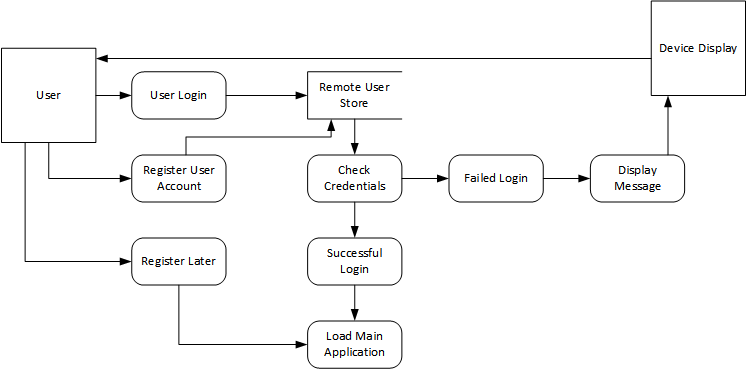
\includegraphics[scale=0.65]{userLoginDFD.png}
\caption{Data Flow Diagram for Logging In and Creating User Accounts}
\label{fig:userLoginDFD}
\end{center}
\end{figure}

Figure~\ref{fig:createTrailDFD} shows the flow of data when a user creates a new trail in the Android application.

\begin{figure}[H]
\begin{center}
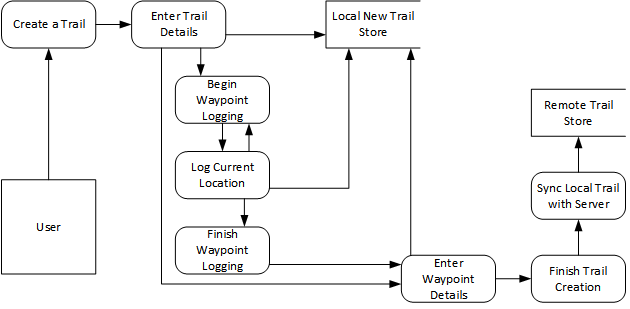
\includegraphics[scale=0.65]{createTrailDFD.png}
\caption{Data Flow Diagram for Creating a New Trail}
\label{fig:createTrailDFD}
\end{center}
\end{figure}


\subsection{User Characteristics}
\label{sec:user-characteristics}

The team has identified multiple types of users for the system:
\begin{description}
\item[Keen Walkers:] The most obvious user. They will likely have some familiarity with the Android operating system as they are capable of installing the application and will be excited to explore trails of varying difficulties.
\item[Primary Schools:] These users are likely to be regular customers with different groups of children. They will be led by a qualified adult, thus reducing the need for the whole group to be well acquainted with the Android operating system.
\item[Heritage Site Admin:] The type of user who will be creating walks for other user to enjoy. The system must be intuitive and, where possible, complete the task of creating a walk in as short a time as possible to help this user.
\end{description}

For all users it is expected that they can read and understand English, they are familiar with the Android operating system and no further familiarity with computer technology shall be assumed.

\subsection{Constraints}
\label{sec:constraints}
As this project has been undertaken as an MEng group project there are multiple teams developing similar applications. The White Rock team have requested that all teams use the same database, the structure of which is to be decided upon between the groups.

\subsection{Assumptions and Dependencies}
\label{sec:assumptions-dependencies}
The assumptions of the project are as follows:

\begin{itemize}
\item Development machines will be available.
\item An Android tablet will be provided for development by White Rock.
\item A server with suitable hardware shall be available for the web portal.
\item Users are available for participation in user studies.
\item Third party libraries have been fully tested.
\item The code-base the team has received from White Rock is of a high enough quality to continue development.
\item All associated costs with web hosting and Google APIs will be covered by White Rock.
\end{itemize}
The dependencies of the project are as follows:
\begin{itemize}
\item The GPS on the tablet is accurate enough to alert users when they are near an item of interest.
\item The GPS is accurate enough to provide directions on time.
\item The database structure is decided upon between teams early into development.
\end{itemize}

\section{Requirements}
\label{sec:requirements}

This section will define the requirements of the software that is to be produced.
Each requirement will be listed with a unique code to allow for easier identification.
These requirements are defined at the request of the client and serve as a binding contract for the delivery of the final product.
The final product must satisfy all requirements listed in this section to fulfil the requirements of the client.
Section \ref{sec:func-reqs} will define the functional requirements of the software, these are requirements that have a specific behaviour or function in the software. 
Section \ref{sec:non-func-reqs} defines the non-functional requirements which specify a criteria which is used to judge the operation of the software.
These can be based on properties such as efficiency, usability and security.
Finally, section \ref{sec:nice-to-have} defines a set of optional features which will be `nice to have'.
These features are not essential to the core functionality of the final product but will add value if they are implemented.
Therefore, these features will be developed if all functional and non-functional requirements have been satisfied and time permits.

\subsection{Functional}
\label{sec:func-reqs}

This section will define the functional requirements for the web portal, android application and database in sections \ref{sec:req-reg-login}, \ref{sec:app-reqs} and \ref{sec:db-reqs} respectively.

\subsubsection{Web Portal}
\label{sec:req-reg-login}

This section defines the requirements of the web portal. 
The web portal will allow users to manage their account, manage created walks and collaborate on other walks.
The web portal will be accessible through a standard web browser where users can log into their personalised account using registered credentials.

\begin{longtable}{|p{2.5cm}p{13cm}|}
\hline
\textbf{Code} & \textbf{Requirement} \\
\hline
WEBREQ1 & The web portal should allow users to register a new account. \\ \hline
WEBREQ2 & The web portal should allow registered users to log in. \\ \hline
WEBREQ3 & The web portal should allow registered users to log out. \\ \hline
WEBREQ4 & The web portal should allow registered users to modify their account details. \\ \hline
WEBREQ5 & The web portal interface should feature distinctive White Rock branding. \\ \hline
WEBREQ6 & The web portal should allow registered users to add sub-branding to created walks. \\ \hline
WEBREQ7 & The web portal should display a registered user's own walks and contributions when logged in. \\ \hline
WEBREQ8 & The web portal should allow registered users to create, edit and delete their own walks. \\ \hline
WEBREQ9 & The web portal should allow registered users to create, edit and delete their own waypoints. \\ \hline
WEBREQ10 & The web portal should allow registered users to add GPS waypoints to a walk. \\ \hline
WEBREQ11 & The web portal should allow registered users to modify the order each waypoint should be visited. \\ \hline
WEBREQ12 & The web portal should allow registered users to upload, edit and delete waypoint data such as images, text, audio and video. \\ \hline
WEBREQ13 & The web portal should allow registered users to provide English and Welsh translation for text. \\ \hline
WEBREQ14 & The web portal should display download statistics for each of the user's walks. \\ \hline
WEBREQ15 & The web portal should display reviews for each of the user's walks. \\ \hline
WEBREQ16 & The web portal should display an average rating for each of the user's walks. \\ \hline
WEBREQ17 & The web portal should notify registered users of waypoint addition requests. \\ \hline
WEBREQ18 & The web portal should allow registered users to accept or reject requested waypoint additions. \\ \hline
WEBREQ19 & The web portal should allow registered users to report bugs and errors. \\ \hline
WEBREQ20 & The web portal should contain an FAQ and user guide. \\ \hline
\end{longtable}

\subsubsection{Android Application}
\label{sec:app-reqs}

This section defines the requirements for the Android application.
Users will download and run the Android application on any Android device.
The Android Application will allow users to explore, rate and comment on user created walks and add way points to their own walks.
Way points will allow users to tag GPS locations and upload associated text, images, video and audio.
User created walks can be downloaded by other users who will be able to access the data associated with each way point in the walk.

\begin{longtable}{|p{2.5cm}p{13cm}|}
\hline
\textbf{Code} & \textbf{Requirement} \\
\hline
APPREQ1 & The application should allow users to register user accounts. \\ \hline
APPREQ2 & The application should allow registered users to log in. \\ \hline
APPREQ3 & The application should allow registered users to log out. \\ \hline
APPREQ4 & The application should allow registered users to modify their account details. \\ \hline
APPREQ5 & The application should allow users to download walks created by registered users. \\ \hline
APPREQ6 & The application should group walks by local area. \\ \hline
APPREQ7 & The application should sort grouped walks by current proximity to the user. \\ \hline
APPREQ8 & The application should allow users to use Google earth and street maps interchangeably while viewing a walk. \\ \hline
APPREQ9 & The application should allow registered users to choose a default map view for a created walk. \\ \hline
APPREQ10 & The application should download data from a remote database. \\ \hline
APPREQ11 & The application should synchronise data whilst the host device is connected to WiFi. \\ \hline
APPREQ12 & The application should give users the option to synchronise data over cellular networks. \\ \hline
APPREQ13 & The application should give users the option to store data on an SD card if available. \\ \hline
APPREQ14 & The application should detect a user's GPS location consistently between devices. \\ \hline
APPREQ15 & The application should display the preferred order to visit waypoints in a walk. \\ \hline
APPREQ16 & The application should display waypoint information even if it has already been visited. \\ \hline
APPREQ17 & The application should allow registered users to create, edit and delete their own walks. \\ \hline
APPREQ18 & The application should allow registered users to tag GPS waypoints in their own walks. \\ \hline
APPREQ19 & The application should track the order GPS waypoints were tagged in a created walk. \\ \hline
APPREQ20 & The application should allow registered users to upload audio, images and video to a waypoint. \\ \hline
APPREQ21 & The application interface should separate audio, images, text and video waypoint data. \\ \hline
APPREQ22 & The application interface should feature distinctive White Rock branding. \\ \hline
APPREQ23 & The application should allow registered users to contribute waypoints to other user's walks by request. \\ \hline
APPREQ24 & The application should allow users to leave reviews on walks. \\ \hline
APPREQ25 & The application should allow users to rate walks they have completed. \\ \hline
APPREQ26 & The application should allow users to report bugs and errors. \\ \hline
APPREQ27 & The application should provide links to the application's Twitter and Facebook channels. \\ \hline
APPREQ28 & The application should provide English and Welsh translations for text. \\ \hline
APPREQ29 & The application should allow users to report inappropriate content to an administrator. \\ \hline
\end{longtable}

\subsubsection{Database Requirements}
\label{sec:db-reqs}

This section defines the requirements for the digital trails database.
The database will store data associated with walks, user accounts and way points.
A local database will reside on user's devices which will mirror a database stored on a remote server.
Only a subset of data from the remote database will be stored on user devices based on the walks that have been downloaded.

\begin{longtable}{|p{2.5cm}p{13cm}|}
\hline
\textbf{Code} & \textbf{Requirement} \\
\hline
DBREQ1 & The database should the ability to store a Walk\\ \hline
DBREQ2 & Each walk should link to a description.  \\ \hline
DBREQ3 & The walks should have `Difficultly', `Duration' and `Distance'. \\ \hline
DBREQ4 & The database should have the ability to store a place, which is a location on a walk.\\ \hline
DBREQ5 & The places should be linked to a walk.\\ \hline
DBREQ6 & The places should have `Latitude' and `Longitude' to store the position. \\ \hline
DBREQ7 & The places should linked to a description. \\ \hline
DBREQ8 & The database should have the ability to store a description for each supported language. \\ \hline
DBREQ9 & The descriptions should be replicas of each other, but in the correct language. \\ \hline
DBREQ10 & The descriptions should include a `Title', a `Short Description' and a `Description'.\\ \hline
DBREQ11 & The database should have the ability to store Photos \\ \hline
DBREQ12 & The database should have the ability to link Photos to places and walks.\\ \hline
DBREQ13 & The photos should store the location of the photo file in the file system.\\ \hline
DBREQ14 & The database should have the abilities to store Videos. \\ \hline
DBREQ15 & The database should have the ability to link Videos to places and walks.\\ \hline
DBREQ16 & The videos should store the location of the video file in the file system.\\ \hline
DBREQ17 & The database should have the ability to store audio. \\ \hline
DBREQ18 & The database should have the ability to link audio to places and walks.\\ \hline
DBREQ19 & The audio should store the location of the audio file in the file system.\\ \hline
DBREQ20 & The database should have the ability to store Users. \\ \hline
DBREQ21 & The users should have a `Username`, an `Email' and a `Password'\\ \hline
DBREQ22 & The users should be linked to Walks, Places, Photos, Videos and Audio they add. \\ \hline
DBREQ23 & The users should store related settings. \\ \hline 

\end{longtable}

\subsection{Non-Functional}
\label{sec:non-func-reqs}

This section defines the non-functional requirements of the software.
These requirements state the properties which are desired of the software.
Such properties include compatibility with different screen sizes; battery and GPS efficiency and that software is usable by colour blind users.

\begin{longtable}{|p{2.5cm}p{13cm}|}
\hline
\textbf{Code} & \textbf{Requirement} \\

\hline
NFREQ1 & The web portal must share the same database as the second development group. \\ \hline
NFREQ2 & The application should be intuitive to users with little technology experience. \\ \hline
NFREQ3 & The application should be usable by colour blind users. \\ \hline
NFREQ4 & The application code should be maintainable for future developers. \\ \hline
NFREQ5 & The application code should be fully documented. \\ \hline
NFREQ6 & The application should run efficiently on lower end GPS-enabled android tablets. \\ \hline
NFREQ7 & The application should run efficiently on android smartphones. \\ \hline
NFREQ8 & The application should be compatible with typical tablet screen sizes. \\ \hline
NFREQ9 & The application should be compatible with typical smartphone screen sizes. \\ \hline
NFREQ10 & The application should be battery efficient by sampling GPS locations based on the user's mode of transport. \\ \hline
NFREQ11 & The application should be bandwidth efficient. \\ \hline
\end{longtable}

\subsection{Nice To Have}
\label{sec:nice-to-have}

This section defines the features which are optional and `nice to have'.
Such features include the integration of Twitter and Facebook channels within the Android application.

\begin{longtable}{|p{2.5cm}p{13cm}|}
\hline
\textbf{Code} & \textbf{Requirement} \\

\hline
NTHREQ1 & A Facebook channel to enable feedback and contributions from users. \\ \hline
NTHREQ2 & A Twitter channel to enable feedback and contributions from users. \\ \hline
NTHREQ3 & The application should display the latest tweets from the Twitter channel. \\ \hline
NTHREQ4 & The application should allow users to advertise their current walk on Facebook and Twitter. \\ \hline
\end{longtable}

\section{Specifications}
\label{sec:specifications}

This section defines the specifications for the functional, non-function and `nice to have' features in sections \ref{sec:func-reqs}, \ref{sec:non-func-specs} and \ref{sec:nice-to-have-specs} respectively.
These specifications describe how the requirements from section \ref{sec:requirements} will be achieved at a high level.
Each software requirement maps to one or more specifications as there may be multiple items needed to achieve a given specification.
Therefore, the specifications will serve as a high level strategy for the implementation of each requirement.

\subsection{Functional}
\label{sec:func-specs}

This section will describe the specifications for the functional requirements defined in section \ref{sec:func-reqs}.

\subsubsection{Web Portal}

The following set of specifications describe how the web portal functional requirements will be achieved.

\begin{longtable}{|p{2.5cm}p{13cm}|}
\hline
\textbf{Code} & \textbf{Specification} \\

\hline
WEBSPEC1 & The web portal will have a `Register' button for users which are not logged in. \\ \hline
WEBSPEC2 & Clicking `Register' will display a view with `Name', `Email Address', `Password', `Password Confirmation' text fields and `Register' and `Cancel' buttons.\\ \hline
WEBSPEC3 & Clicking `Cancel' will return the user to the index page.\\ \hline
WEBSPEC4 & Clicking `Register' will create a user, log them in and email them a confirmation. \\ \hline
WEBSPEC5 & There will be a `Login' link on for users that are not logged in.\\ \hline
WEBSPEC6 & Clicking `Login' will present a pop up with `Username' and `Password' fields and `Login' and `Cancel' buttons. \\ \hline
WEBSPEC7 & Clicking `Login' will create an authenticated session for the user stored in a temporary cookie.\\ \hline
WEBSPEC8 & Clicking `Cancel' will dismiss the popup. \\ \hline
WEBSPEC9 & When users are logged in they will be presented with a `Logout' link\\ \hline
WEBSPEC10 & Clicking `Logout' will delete the session cookie and return them to the index page as guest. \\ \hline
WEBSPEC11 & The web portal will feature an `Edit Account' button. \\ \hline
WEBSPEC12 & Clicking the `Edit Account' will display a view that allows the user to edit their `full name, email and password', a `cancel' button and a `save' button. \\ \hline
WEBSPEC13 & Clicking the `Save' button will validate the full name, email and password text boxes. If successful, a notification will inform the user that changes were made to their details. \\ \hline
WEBSPEC14 & Clicking the `Cancel' button will cancel current changes made to the user`s details. \\ \hline
WEBSPEC15 & All web portal views will feature the company logo and use a house colour scheme. \\ \hline
WEBSPEC16 & The `user account settings' view will feature a company branding tab, allowing the user to attach their company logo to a walk. \\ \hline
WEBSPEC17 & The company branding tab will feature a `Browse' button, allowing the user to browse their computer for a particular image and will feature a `Save' button, allowing the user to upload their image. \\ \hline
WEBSPEC18 & Successfully logging in will take the user to a `Homepage' view featuring their own walks and contributions. \\ \hline
WEBSPEC19 & The web portal will feature a `Walk' button on its side bar. \\ \hline
WEBSPEC20 & Clicking the `Walk' button will navigate the user to a view featuring a list of walks and an `Add walk' button. \\ \hline
WEBSPEC21 & Clicking the `Add walk' button will display a view featuring `Walk name, description' textboxes, `Cancel' and `Create' button. \\ \hline
WEBSPEC22 & The `Walk name' and `Description' text boxes will include a profanity filter, preventing inappropriate words being used. \\ \hline
WEBSPEC23 & Clicking the `Cancel' button will navigate the user back to the `Homepage' view. \\ \hline
WEBSPEC24 & Clicking the `Create' button will create a new walk. \\ \hline
WEBSPEC25 & The walk list view will feature an `Edit' button and `Delete' button adjacent to each walk. \\ \hline
WEBSPEC26 & Clicking the `Edit' button will navigate to a view where the user can edit the `Walk name, description' text boxes. \\ \hline
WEBSPEC27 & Clicking the `Delete' button will display a view, asking the user to confirm they wish to delete the walk. \\ \hline
WEBSPEC28 & When in user-walk list view, clicking on a walk will display a view featuring a list of walk waypoints and an `Add waypoint' button. \\ \hline
WEBSPEC29 & Clicking the `Add waypoint' button will display a view featuring `Waypoint name', `Waypoint description' text boxes, `Location Map', `Add image', `Add video' and `Add audio'. \\ \hline
WEBSPEC30 & Clicking the `Add image' button will display a `Browse', `Add' and `Cancel' button. \\ \hline
WEBSPEC31 & Clicking the `Browse' button will allow the user to browse their computer for a suitable image of the waypoint. \\ \hline
WEBSPEC32 & Clicking the `Save' button will upload the image to the waypoint. \\ \hline
WEBSPEC33 & Clicking the `Cancel' button will navigate the user back to the waypoint view. \\ \hline
WEBSPEC34 & Clicking the `Add video' button will display a `Browse', `Add' and `Cancel' button. \\ \hline
WEBSPEC35 & Clicking the `Browse' button will allow the user to browse their computer for a suitable video of the waypoint. \\ \hline
WEBSPEC36 & Clicking the `Save' button will upload the video to the waypoint. \\ \hline
WEBSPEC37 & Clicking a specific point on the `Location map' of the walk will place a waypoint based on its geological location. \\ \hline
WEBSPEC38 & The longitude and latitude co-ordinates must be accepted in the following formats: `British Grid', `Decimal degrees', `Degrees minutes and seconds' and `Degrees and decimal minutes'. \\ \hline
WEBSPEC39 & The waypoint list view will feature an `Edit' button and a `Delete' button adjacent to each waypoint. \\ \hline
WEBSPEC40 & Clicking the `Edit waypoint' button will navigate to a view where the user can edit the `Waypoint name, description' textboxes, waypoint image, waypoint video, waypoint audio and waypoint geological location. \\ \hline
WEBSPEC41 & Each feature of a waypoint shall include a delete button adjacent to the feature. \\ \hline
WEBSPEC42 & Clicking the `Delete' button of a waypoint feature will display a view asking the user if they wish to delete it. For example, clicking the delete button adjacent to the waypoint video will ask the user if they wish to delete the video. \\ \hline
WEBSPEC43 & Clicking the `Delete waypoint' will display a view, asking the user to confirm they wish to delete the waypoint. \\ \hline
WEBSPEC44 & The waypoints view will feature a `Change order' button. \\ \hline
WEBSPEC45 & Clicking the `Change order' button will display a list view of the waypoints, an `Up' button and a `Down' button. \\ \hline
WEBSPEC46 & When a waypoint is selected, clicking the `Up' button will move the waypoint up the list order, clicking the `Down' button will move the waypoint down the list order. \\ \hline
WEBSPEC47 & The web portal side bar will feature a `Translate' button that will display a view featuring `Welsh' and `English' buttons. \\ \hline
WEBSPEC48 & Clicking the `Welsh' button will translate the text into English. \\ \hline
WEBSPEC49 & Clicking the `English' button will translate the text into Welsh. \\ \hline
WEBSPEC50 & The web portal side bar will feature a `Statistics' button, a `Ratings' button, a `Review' button, a `Requests' and a `Report' button. \\ \hline
WEBSPEC51 & Clicking the `Statistics' button navigates the user to a statistics view, displaying each of the user's walks and their download history. \\ \hline
WEBSPEC52 & Clicking the `Ratings' button navigates the user to a ratings view, displaying each of the user's walks and average ratings. \\ \hline
WEBSPEC53 & Clicking the `Reviews' button navigates the user to a review view, displaying each of the user's walks a list of reviews. \\ \hline
WEBSPEC54 & Clicking on the `Request' button navigates the user to a request view, displaying pending waypoints to be added to one of their walks. \\ \hline
WEBSPEC55 & Clicking on a pending waypoint will display a view featuring an `Accept' or `Reject' button. \\ \hline
WEBSPEC56 & Clicking the `Accept' button will add the waypoint to the walk. \\ \hline
WEBSPEC57 & Clicking the `Reject' button will delete the waypoint request. \\ \hline
WEBSPEC58 & Clicking the `Report' button will display a report view, featuring a report/bug `Name', `Description' textboxes, `Send' button and `Cancel' button. \\ \hline
WEBSPEC59 & Clicking the `Send' button will file a report to the White Rock maintenance team. \\ \hline
WEBSPEC60 & Clicking the `Cancel' button will navigate the user to the homepage. \\ \hline
WEBSPEC61 & Clicking the `FAQ' button will navigate to the FAQ. \\ \hline
WEBSPEC62 & The FAQ page shall contain two panels, one for links to question, on the left, and one for answers, on the right. \\ \hline
WEBSPEC63 & The web portal shall have a `Guide' button which links to the User Guide. \\ \hline
WEBSPEC64 & The User Guide page shall contain two panels, one for the contents page, on the left, and one for the guide, on the right. \\ \hline
WEBSPEC65 & The User Guide page will update the guide when the user clicks a link in the contents panel.  \\ \hline
WEBSPEC66 & The User Guide guide panel will contain a back and next button to change the content in the panel. \\ \hline
\end{longtable}

\subsubsection{Android Application}

The following set of specifications describe how the Android application functional requirements will be achieved.

\begin{longtable}{|p{2.5cm}p{13cm}|}
\hline
\textbf{Code} & \textbf{Specification} \\

\hline
APPSPEC1 & The application's login view will feature a `Register' button. \\ \hline
APPSPEC2 & Clicking the `Register' button will display a view featuring full name, email and password text boxes, `Register' and `Cancel' buttons. \\ \hline
APPSPEC3 & Clicking the `Register' button will validate the full name, email and password text boxes. If successful, the account will be created, user logged in and navigate the user to a personal home view. \\ \hline
APPSPEC4 & Clicking the `Cancel' button will cancel the registration process and navigate the user back to the launch view. \\ \hline
APPSPEC5 & The application's launch view will feature a `Login' button. \\ \hline
APPSPEC6 & Clicking the `Login' button will display a login view featuring email and password text boxes, `Sign In' and `Cancel' buttons. \\ \hline
APPSPEC7 & Clicking the `Sign In' button will validate the email and password text boxes, log the user in and navigate to a personal home view if successful. \\ \hline
APPSPEC8 & Clicking the `Cancel' button will cancel the sign in process and navigate the user back to the launch view. \\ \hline
APPSPEC9 & The personal home view and options menu will feature a `Log Out' button. \\ \hline
APPSPEC10 & Clicking the `Log Out' button will log the user out of the application and navigate to the launch view. \\ \hline
APPSPEC11 & The personal home view and options menu will feature an `Account' button. \\ \hline
APPSPEC12 & Clicking the `Account' button will navigate the user to a view featuring full name, email, password text boxes and `Save', `Cancel' buttons. \\ \hline
APPSPEC13 & Clicking the `Save' button will validate the full name, email, password text boxes and save any changes to the user's account if successful. A notification will be displayed to inform the user of success or failure. \\ \hline
APPSPEC14 & Clicking the `Cancel' button will cancel the process of account modification and navigate the user to the personal home view. \\ \hline
APPSPEC15 & The launch view will feature a `Search' button which is enabled only when the application detects a WiFi connection. \\ \hline
APPSPEC16 & Clicking the `Search' button will navigate the user to a view containing a search text box, `Go' button and list of walks. \\ \hline
APPSPEC17 & Clicking the `Go' button will filter the walk list to display only the walk names with a full or partial match to the search text. \\ \hline
APPSPEC18 & Walk list items will display the walk name, author, partial description, user rating, downloads and `Download' button. \\ \hline
APPSPEC19 & Clicking the `Download' button will download the walk to the user's device and replace the button with a `tick' icon. \\ \hline
APPSPEC20 & The application will group walk list items which are close in proximity together in a sublist with a heading name of the common local area. \\ \hline
APPSPEC21 & Walk list items grouped by local area will be displayed in descending order based on closest proximity to the application user. \\ \hline
APPSPEC22 & An options menu will feature `Google Earth' and `Google Street' buttons which will be accessible whilst viewing a walk. \\ \hline
APPSPEC23 & Clicking the `Google Earth' button will change the current walk's map to the Google Earth view. \\ \hline
APPSPEC24 & Clicking the `Google Street' button will change the current walk's map to the Google Street view. \\ \hline
APPSPEC25 & Walk edit and add views will feature a default map drop down box containing the options `Google Earth' and `Google Street'. \\ \hline
APPSPEC26 & Application data will be downloaded through a web API interfacing a remote database which will be hosted on a Linux server.  \\ \hline
APPSPEC27 & Application data will be synchronised with a remote database when the application is launched and the device is connected to WiFi. \\ \hline
APPSPEC28 & The application will display a loading view whilst synchronising application data. \\ \hline
APPSPEC29 & The application will feature a settings view containing a toggle button to enable data download over the cellular data network. \\ \hline
APPSPEC30 & Clicking the toggle button will change its state to on or off accordingly and the setting will be saved. \\ \hline
APPSPEC31 & The settings view will feature a drop down box containing the storage options `Internal' and `SD Card'. \\ \hline
APPSPEC32 & Selecting an option from the storage drop down box will save the setting and move data to the chosen location if it has changed. \\ \hline
APPSPEC33 & The application will display a loading view whilst moving application data to a different location. \\ \hline
APPSPEC34 & A location strategy will be re-implemented using the Android location services API. \\ \hline
APPSPEC35 & The application's GPS accuracy will be tested on the target Hudl tablet and a low end Android 2.2 mobile device to ensure consistency. \\ \hline
APPSPEC36 & The walk view will place a graphic over each waypoint on the map containing a number to represent it's preferred visit order. \\ \hline
APPSPEC37 & The walk view will highlight the next waypoint to visit using a different graphic colour. \\ \hline
APPSPEC38 & Waypoint information will be displayed to the user even if the waypoint has previously been visited since the walk view was opened. \\ \hline
APPSPEC39 & The application will feature a `Walk Options' button.\\ \hline
APPSPEC40 & Clicking on the `Walk Options' button will display a view with `Create Walk' button and a list of walks owned by the user. \\ \hline
APPSPEC41 & Each walk in the list will have an `Edit' and `Delete' button.\\ \hline
APPSPEC42 & Clicking the `Create Walk' button will display a view with `walk name, description' text boxes and `Add waypoints', `Create' and `Cancel' buttons.\\ \hline
APPSPEC43 & Pressing an `Edit' button on a walk will bring up the `Edit Walks' view where the user can edit the `Walk name' and `Description' text fields. There will be an `Add waypoint', `Edit Waypoints', `Create' and `Cancel' buttons. \\ \hline
APPSPEC44 & Pressing the `Delete' button will display a model asking the user to confirm the deletion. \\ \hline
APPSPEC45 & Pressing an `Add waypoints' button will bring up a map view where the users can zoom in and move around. Waypoints are positioned by pressing on a location for a couple of seconds. \\ \hline
APPSPEC46 & Waypoints are automatically assigned the order in which they were created. \\ \hline
APPSPEC47 & Once a location has been assigned the `Edit Waypoint' view is displayed.\\ \hline
APPSPEC48 & Pressing the `Edit Waypoints' button will display a list of current waypoints. Each waypoint will have a `Edit' and `Delete' button. \\ \hline
APPSPEC49 & Pressing the `Edit' button will display an `Edit Waypoint' view. \\ \hline
APPSPEC50 & Pressing the `Delete' button will display a model asking the user to confirm the deletion of the waypoint. \\ \hline
APPSPEC51 & The `Edit Waypoints' view displays a map thumbnail of the location, `Name' and `Description' text boxes, an `Upload' button to add images, audio and video, and a gallery of uploaded media. \\ \hline
APPSPEC52 & Pressing on an item in the gallery of uploaded media will show a pop-up model with a `Delete' button. Clicking `Delete' will present another model asking the user to confirm the deletion. \\ \hline
APPSPEC53 & When viewing a waypoint there will be tabs for 'Descriptions', 'Images', 'Audio' and 'Videos'. \\ \hline
APPSPEC54 & Pressing the map thumbnail will allow the user to change the position of the waypoint. It will show a map with a movable point and `Confirm' and `Cancel' buttons. \\ \hline
APPSPEC55 & The application will feature White Rock branding and designs where appropriate to build the brand image. \\ \hline
APPSPEC56 & When a registered user is viewing a walk there will be an `Edit' button \\ \hline
APPSPEC57 & Pressing the `Edit' button will display the `Edit Walks' view. The `walk name' and `description' fields will be greyed out to prevent editing.\\ \hline
APPSPEC58 & Any edits to walks created by people other than owner will require them to be confirmed by the owner before being published. \\ \hline
APPSPEC59 & When a user has visited every waypoint on a walk a model will appear asking the user if they have finished. It will have `Finished' and `Carry on' buttons. \\ \hline
APPSPEC60 & A user can force a walk to finish by pressing a `Finish' button in the options menu. \\ \hline
APPSPEC61 & Pressing `Finish' displays a view with a `Review' text box, `Submit review' button, 5 star rating system and `Report a bug' button. \\ \hline
APPSPEC62 & Submitting a review submits the data in the `Review' text box and displays it on the walks information page.\\ \hline
APPSPEC63 & Filling in the 5 star rating system will automatically send the result to the server.\\ \hline
APPSPEC64 & Pressing `Report a Bug' will launch the email client. \\ \hline
APPSPEC65 & The `to? address will be set as the email address of the owner, the `subject? field will be set in the format ``BUG REPORT - WALK `NAME' ''.\\ \hline
APPSPEC66 & The application will link to the White Rocks Twitter and Facebook page from the main page.\\ \hline
APPSPEC67 & The application provide an option in the settings view to display welsh text where available. \\ \hline
APPSPEC68 & On each waypoint and walk there will be a `Report' button which will flag the content as inappropriate. \\ \hline
APPSPEC69 & And content which has been flagged as inappropriate will appear to administrators, who can modify or delete it. \\ \hline
\end{longtable}

\subsubsection{Database Specifcation}

\begin{longtable}{|p{2.5cm}p{13cm}|}
\hline
\textbf{Code} & \textbf{Specification} \\
\hline
DBSPEC1 & The database will have have a Walks table\\ \hline
DBSPEC2 & Every table will have have an `ID' field as its primary key.\\ \hline
DBSPEC3 & The walks table will have have a `DescriptionID' field to relate to a row in a description table. \\ \hline
DBSPEC4 & The walks table will have have `Difficultly',  `Duration' and `Distance' field. \\ \hline
DBSPEC5 & The walks table will have a `UserID' field to relate to the specific user who created it. \\ \hline
DBSPEC6 & The database will have have a Place table to store locations on a walk.\\ \hline
DBSPEC7 & The places table will have have a `WalkID' field to relate to a row in the walks table.\\ \hline
DBSPEC8 & The places table will have have `Latitude' and `Longitude'  fields to store the position. \\ \hline
DBSPEC9 & The places table will have have a `DescriptionID' field to relate to a row in a description table. \\ \hline
DBSPEC10 & The places table will have a `UserID' field to relate to a specific user who created it. \\\hline
DBSPEC11 & The database will have have a Description table for each supported language. \\ \hline
DBSPEC12 & The description tables will have be replicas of each other, but in the correct language. \\ \hline
DBSPEC13 & The description tables will have have `Title', `Short Description' and `Description' fields.\\ \hline
DBSPEC14 & The description tables will have a `UserID' field to relate to a specific user who created it. \\\hline
DBSPEC15 & The database will have have a Photos table.\\ \hline
DBSPEC16 & The photos table will have have a `placeID' field to relate to a row in the Places table. \\ \hline
DBSPEC17 & The photos table will have have a `walkID' field to relate to a row in the walks table.\\ \hline
DBSPEC18 & The photos table will have have a `Location' field to store the location of the photo file in the file system.\\ \hline
DBSPEC19 & The photos table will have a `UserID' field to relate to a specific user who created it. \\\hline
DBSPEC20 & The database will have have a Videos table. \\ \hline
DBSPEC21 & The videos table will have have a `placeID' field to relate to a row in the Places table. \\ \hline
DBSPEC22 & The videos table will have have a `walkID' field to relate to a row in the walks table.\\ \hline
DBSPEC23 & The videos table will have have a `Location' field to store the location of the video file in the file system.\\ \hline
DBSPEC24 & The videos table will have a `UserID' field to relate to a specific user who created it. \\\hline
DBSPEC25 & The database will have have a Audio table. \\ \hline
DBSPEC26 & The audio table will have have a `placeID' field to relate to a row in the Places table. \\ \hline
DBSPEC27 & The audio table will have have a `walkID' field to relate to a row in the walks table.\\ \hline
DBSPEC28 & The audio table will have have a `Location' field to store the location of the audio file in the file system.\\ \hline
DBSPEC29 & The audio table will have a `UserID' field to relate to a specific user who created it. \\\hline
DBSPEC30 & The database will have a  Users table \\ \hline
DBSPEC31 & The users table will have `Username', `Email' and `Password' fields.\\ \hline
DBSPEC32 & The users table will have fields to store adequate user settings. \\ \hline



\end{longtable}

\subsection{Non-Functional}
\label{sec:non-func-specs}

This section will describe the specifications for the non-functional requirements defined in section \ref{sec:non-func-reqs}.

\begin{longtable}{|p{2.5cm}p{13cm}|}
\hline
\textbf{Code} & \textbf{Specification} \\

\hline
NFSPEC1 & Database schema shall be agreed with the second development group \\ \hline
NFSPEC2 & The final database will be hosted on a central server. \\ \hline
NFSPEC3 & The user interface shall be well labelled. \\ \hline
NFSPEC4 & The user will follow traditional mobile interface design decisions to reduce the learning curve of the application. \\ \hline
NFSPEC5 & Use the interface of default Android applications where possible. e.g. The Holo-light theme \\ \hline
NFSPEC6 & Create an optional step by step tutorial for first time users. \\ \hline
NFSPEC7 & Create button to access the tutorial in the settings screen. \\ \hline
NFSPEC8 & In the settings view there will be an option to enable colour blind mode. \\ \hline
NFSPEC9 & Colour blind mode will modify the user interface to use a colour palette usable by the majority of colour blind users. \\ \hline
NFSPEC10 & In the settings view there will be an option to enable a speech to text feature. \\ \hline
NFSPEC11 & The speech to texture feature will turn user submitted audio into on-screen text. \\ \hline
NFSPEC12 & The settings view will contain an option to allow the device to vibrate when approaching a destination along the route. \\ \hline
NFSPEC13 & The settings view will contain an option to allow the device to emit an audible beep when approaching a destination along the route. \\ \hline
NFSPEC14 & Coding conventions shall be enforced. \\ \hline
NFSPEC15 & Unit tests shall be ran and results documented during development. \\ \hline
NFSPEC16 & All code shall be commented, according to conventions. \\ \hline
NFSPEC17 & Code documentation shall be generated by Doxygen. \\ \hline
NFSPEC18 & Compile with Android 2.2 as a minimum Operating System. \\ \hline
NFSPEC19 & Use compatibility libraries to allow for compatibility for both low and high end devices. \\ \hline
NFSPEC20 & Create a dynamic user interface using Fragments. \\ \hline
NFSPEC21 & Sample GPS based on mode of transport the user has input. (update when better idea). \\ \hline
\end{longtable}

\subsection{Nice To Have}
\label{sec:nice-to-have-specs}

This section will describe the specifications for the `nice to have' requirements defined in section \ref{sec:nice-to-have}.

\begin{longtable}{|p{2.5cm}p{13cm}|}
\hline
\textbf{Code} & \textbf{Specification} \\

\hline
NTHSPEC1 & A Facebook page for the digital trails application will be created to promote the application and enable community feedback. \\ \hline
NTHSPEC2 &  A Twitter page for the digital trails application will be created to promote the application and enable community feedback. \\ \hline
NTHSPEC3 & The Twitter API will be used to access tweets from the application's Twitter page. \\ \hline
NTHSPEC4 & The Facebook API will be used to allow sharing to user Facebook accounts. \\ \hline
NTHSPEC5 & Allow users to link their accounts to their Facebook accounts. \\ \hline
\end{longtable}


\section{Cross References}
\label{sec:cross-refs}

This section will cross reference each requirement to one or more specifications which describe how they will be achieved.
Requirements are mapped to specifications by their assigned unique identification codes.
A requirement can be considered to be satisfied when each of its corresponding specifications have been implemented.

\subsection{Functional}

This section will define cross reference mappings from the web portal and android application function requirements to corresponding sets of specifications.

\subsubsection{Web Portal}

\begin{longtable}{|p{2.7cm}|p{10cm}|}
\hline
\textbf{Requirement Code} & \textbf{Specification Code} \\

\hline
{WEBREQ1} &
{WEBSPEC1, WEBSPEC2, WEBSPEC3, WEBSPEC4}\\\hline
{WEBREQ2} &
{WEBSPEC5, WEBSPEC6, WEBSPEC7, WEBSPEC8}\\\hline
{WEBREQ3} &
{WEBSPEC9, WEBSPEC10}\\\hline
{WEBREQ4} &
{WEBSPEC11, WEBSPEC12, WEBSPEC13, WEBSPEC14}\\\hline
{WEBREQ5} &
{WEBSPEC15}\\\hline
{WEBREQ6} &
{WEBSPEC16, WEBSPEC17}\\\hline
{WEBREQ7} &
{WEBSPEC18, WEBSPEC19}\\\hline
{WEBREQ8} &
{WEBSPEC20, WEBSPEC21, WEBSPEC22, WEBSPEC23, WEBSPEC24, WEBSPEC25, WEBSPEC26, WEBSPEC27,
WEBSPEC28}\\\hline
{WEBREQ9} &
{WEBSPEC29, WEBSPEC30, WEBSPEC31, WEBSPEC32, WEBSPEC33, WEBSPEC34, WEBSPEC35, WEBSPEC36, WEBSPEC37,
WEBSPEC38, WEBSPEC39, WEBSPEC40, WEBSPEC44}\\\hline
{WEBREQ10} &
{WEBSPEC38, WEBSPEC39, WEBSPEC41}\\\hline
{WEBREQ11} &
{WEBSPEC45, WEBSPEC46, WEBSPEC47}\\\hline
{WEBREQ12} &
{WEBSPEC41, WEBSPEC42, WEBSPEC43}\\\hline
{WEBREQ13} &
{WEBSPEC48, WEBSPEC49, WEBSPEC50}\\\hline
{WEBREQ14} &
{WEBSPEC51, WEBSPEC52}\\\hline
{WEBREQ15} &
{WEBSPEC53}\\\hline
{WEBREQ16} &
{WEBSPEC54}\\\hline
{WEBREQ17} &
{WEBSPEC55}\\\hline
{WEBREQ18} &
{WEBSPEC56, WEBSPEC57, WEBSPEC58}\\\hline
{WEBREQ19} &
{WEBSPEC59, WEBSPEC60, WEBSPEC61}\\\hline
{WEBREQ20} &
{WEBSPEC62, WEBSPEC63, WEBSPEC64, WEBSPEC65, WEBSPEC66, WEBSPEC67}\\\hline 
\end{longtable}


\subsubsection{Android Application}

\begin{longtable}{|p{2.7cm}|p{10cm}|}
\hline
\textbf{Requirement Code} & \textbf{Specification Code} \\
\hline
{APPREQ1} &
{APPSPEC1, APPSPEC2, APPSPEC3, APPSPEC4}\\\hline
{APPREQ2} &
{APPSPEC5, APPSPEC6, APPSPEC7, APPSPEC8}\\\hline
{APPREQ3} &
{APPSPEC9, APPSPEC10}\\\hline
{APPREQ4} &
{APPSPEC11, APPSPEC12, APPSPEC13, APPSPEC14}\\\hline
{APPREQ5} &
{APPSPEC15, APPSPEC16, APPSPEC17, APPSPEC18, APPSPEC19, }\\\hline
{APPREQ6} &
{APPSPEC20}\\\hline
{APPREQ7} &
{APPSPEC21}\\\hline
{APPREQ8} &
{APPSPEC22, APPSPEC23, APPSPEC24}\\\hline
{APPREQ9} &
{APPSPEC25}\\\hline
{APPREQ10} &
{APPSPEC26}\\\hline
{APPREQ11} &
{APPSPEC27, APPSPEC28}\\\hline
{APPREQ12} &
{APPSPEC29, APPSPEC30}\\\hline
{APPREQ13} &
{APPSPEC31, APPSPEC32, APPSPEC33}\\\hline
{APPREQ14} &
{APPSPEC34, APPSPEC35}\\\hline
{APPREQ15} &
{APPSPEC36, APPSPEC37}\\\hline
{APPREQ16} &
{APPSPEC38}\\\hline
{APPREQ17} &
{APPSPEC39, APPSPEC40, APPSPEC41, APPSPEC42, APPSPEC43, APPSPEC44, APPSPEC45}\\\hline
{APPREQ18} &
{APPSPEC45, APPSPEC47, APPSPEC48, APPSPEC49, APPSPEC50, APPSPEC54}\\\hline
{APPREQ19} &
{APPSPEC46}\\\hline
{APPREQ20} &
{APPSPEC51, APPSPEC52}\\\hline
{APPREQ21} &
{APPSPEC53}\\\hline
{APPREQ22} &
{APPSPEC55}\\\hline
{APPREQ23} &
{APPSPEC56, APPSPEC57, APPSPEC58}\\\hline
{APPREQ24} &
{APPSPEC59, APPSPEC60, APPSPEC61, APPSPEC62}\\\hline
{APPREQ25} &
{APPSPEC61, APPSPEC63}\\\hline
{APPREQ26} &
{APPSPEC61, APPSPEC64, APPSPEC65}\\\hline
{APPREQ27} &
{APPSPEC66}\\\hline
{APPREQ28} &
{APPSPEC67}\\\hline
{APPREQ29} &
{APPSPEC68, APPSPEC69}\\\hline
\end{longtable}

\subsubsection{Database}

\begin{longtable}{|p{2.7cm}|p{10cm}|}
\hline
\textbf{Requirement Code} & \textbf{Specification Code} \\
\hline
{DBREQ1} &
{DBSPEC1, DBSPEC2}\\\hline
{DBREQ2} &
{DBSPEC3}\\\hline
{DBREQ3} &
{DBSPEC4}\\\hline
{DBREQ4} &
{DBSPEC6, DBSPEC7, DBSPEC2}\\\hline
{DBREQ5} &
{DBSPEC7}\\\hline
{DBREQ6} &
{DBSPEC8}\\\hline
{DBREQ7} &
{DBSPEC9}\\\hline
{DBREQ8} &
{DBSPEC11, DBSPEC2}\\\hline
{DBREQ9} &
{DBSPEC12}\\\hline
{DBREQ10} &
{DBSPEC13}\\\hline
{DBREQ11} &
{DBSPEC15, DBSPEC2}\\\hline
{DBREQ12} &
{DBSPEC13}\\\hline
{DBREQ13} &
{DBSPEC16, DBSPEC17}\\\hline
{DBREQ14} &
{DBSPEC18}\\\hline
{DBREQ15} &
{DBSPEC20, DBSPEC2}\\\hline
{DBREQ16} &
{DBSPEC21, DBSPEC22}\\\hline
{DBREQ17} &
{DBSPEC23}\\\hline
{DBREQ18} &
{DBSPEC25, DBSPEC2}\\\hline
{DBREQ19} &
{DBSPEC26, DBSPEC27}\\\hline
{DBREQ20} &
{DBSPEC28}\\\hline
{DBREQ21} &
{DBSPEC30}\\\hline
{DBREQ22} &
{DBSPEC5, DBSPEC10, DBSPEC14, DBSPEC19, DBSPEC24, DBSPEC29}\\\hline
{DBREQ23} &
{DBSPEC32}\\\hline
\end{longtable}


\subsection{Non-Functional}

This section will define cross reference mappings from non-function requirements to a set of satisfying specifications.

\begin{longtable}{|p{2.7cm}|p{10cm}|}
\hline
\textbf{Requirement Code} & \textbf{Specification Code} \\

\hline 
{NFREQ1} &
{NFSPEC1, NFSPEC2}\\\hline
{NFREQ2} &
{NFSPEC3, NFSPEC4, NFSPEC5, NFSPEC6, NFSPEC7}\\\hline
{NFREQ3} &
{NFSPEC8, NFSPEC9, NFSPEC10, NFSPEC11, NFSPEC12, NFSPEC13}\\\hline
{NFREQ4} &
{NFSPEC14, NFSPEC15, NFSPEC16, NFSPEC17}\\\hline
{NFREQ5} &
{NFSPEC16, NFSPEC17}\\\hline
{NFREQ6} &
{NFSPEC18, NFSPEC19}\\\hline
{NFREQ7} &
{NFSPEC18, NFSPEC19}\\\hline
{NFREQ8} &
{NFSPEC20}\\\hline
{NFREQ9} &
{NFSPEC20}\\\hline
{NFREQ10} &
{NFSPEC21}\\\hline
{NFREQ11} &
{NFSPEC21}\\\hline
\end{longtable}

\subsection{Nice To Have}

This section will define cross reference mappings from nice-to-have requirements to a set of satisfying specifications.

\begin{longtable}{|p{2.7cm}|p{10cm}|}
\hline
\textbf{Requirement Code} & \textbf{Specification Code} \\

\hline 
{NTHREQ1} &
{NTHSPEC1}\\\hline
{NTHREQ2} &
{NTHSPEC2}\\\hline
{NTHREQ3} &
{NTHSPEC3}\\\hline
{NTHREQ4} &
{NTHSPEC4, NTHSPEC5}\\\hline
\end{longtable}

\section{Methodology}
\label{sec:methodologies}
The chosen methodology must be suited to a small team working closely with the client. As the application is to be used by a wide array of people with varying levels of technical competency regular, high quality feedback will be necessary to ensure a positive user experience. From this it can be seen that an agile development methodology is likely to be most appropriate. In section~\ref{sec:considered-methods} the range of methodologies considered can be seen. In section~\ref{sec:chosen-method} the chosen methodology can be seen.

\subsection{Considered Methodologies}
\label{sec:considered-methods}
\subsubsection{Spiral}
This section is a modified version of the work found in ``A RESTful Document Archival System''~\cite{restWeb}. The spiral methodology is a risk based system, which works iteratively towards a final working project. The process derives its name from the pattern with which its process follows. There are 4 basic activities which must occur in cycle loop of the spiral~\ref{fig:spiral}. These are:

\begin{enumerate}
  \item Consider all success-critical win conditions.
  \item Identify and evaluate alternative methods for meeting win conditions.
  \item Identify and resolve risks caused by the methods for meeting win conditions. 
  \item Obtain the approval of stakeholders and their commitment to the next cycle. 
\end{enumerate}

\begin{figure}[H]
\begin{center}
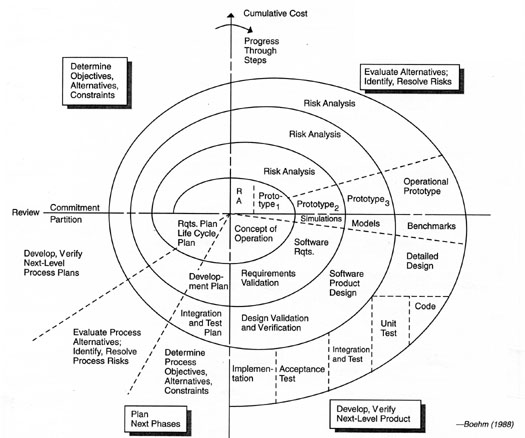
\includegraphics[scale=2.5]{spiral.jpeg}
\label{fig:spiral}
\caption{The spiral model \cite{spiral}}
\end{center}
\end{figure}

By identifying risks at each cycle the model allows the developers to decide on the best approach for that cycle and minimise the chance of failure through correct mitigation of those risks. 

This model requires the use of iterative development techniques. This helps force developers to make improvements to previous implementations and requirements, but the exact nature of the iterations are down to interpretation based upon the risks of the project.

Over all spiral is provides a good way of minimising risks in a project but it also has its down sides. It is possible that it it could be executed as simple cycle of waterfall development, this is not the intended use of the the project and is rarely the correct thing to do for the given risks of a project. It could also create an overly complex development strategy which becomes confusing to the development team. This complexity is one of the main arguments against the Spiral model and is addressed by other more agile methods. 

\subsubsection{Prototyping}
The prototyping methodology attempts to improve the flaws found in traditional software development models in which the product is not tested to see if it meets requirements until the end of the project. The prototyping process has four steps:
\begin{enumerate}
\item Identify basic requirements.
\item Develop initial prototype.
\item Review.
\item Revise and Enhance the prototype.
\end{enumerate}

A prototype is in one of two dimensions:
\begin{description}
\item[Horizontal] A user interface prototype which provides a broad view of the system from a user interface perspective. 
\item[Vertical] A complete prototype of a single subsystem or function.
\end{description}

There are many types of prototyping:
\begin{description}
\item[Throwaway] The creation of a temporary prototype, which will be thrown away, used to demonstrate how requirements might look when implemented into the final system. This allows for quick feedback from the user. Once the requirements have been finalised via prototyping, a set of final requirements are written and development of the final product begins.
\item[Evolutionary] Entails the creation of a robust prototype which will be constantly improved. The prototype is the heart of the system upon which new features can be added. The philosophy behind this approach is that a product is never done, but ``always maturing as the usage environment changes''~\cite{spcPrototyping}.
\item[Incremental] Requirements are developed as separate prototypes before being combined as the final design.
\item[Extreme] Especially used in web development. It is not discussed here as it is not applicable to the majority of the project.
\end{description}

The key benefits of prototyping as a methodology are a reduction in time and costs as changes to the prototypes are cheap in comparison to attempting to change the end product. There is also an increase in involvement between the development team and the user, allowing for faster feedback which will lead to a product the customer is satisfied with.

The disadvantages involve insufficient analysis, where developers spend too much time focusing on limited prototypes to see the bigger picture of the final application, often seeing developers overlook better solutions. Developers may also become attached to a prototype, over-estimate the ease at which a prototype may be implemented and develop the prototype excessively instead of moving on to the next stage.

\subsubsection{Extreme Programming}
This section has been taken, verbatim, from ``FormulaVis: System Requirements Specification''~\cite{formulaVis}. Extreme Programming is an agile development model aimed at improving the software quality by ensuring a fast and efficient response to changing requirements.

This model advocates frequent releases, similar to sprints in the SCRUM model, which improve productivity and create checkpoints where requirements can be reviewed and adapted. Other elements include pair programming, code reviews and unit testing of all code. Features should not be developed, in this model, until they are needed.

Development cycles begin with a Planning Game, a meeting that occurs at the begin of each cycle. This is divided into two tasks, release planning which determines the requirements to be included in this cycle and when the cycle should end. This phase includes the customer. The second phase is the iteration planning phase, in this phase the requirements are translated into tasks and assigned to programmers. These are then completed before the end of the cycle.

During implementation programmers usually work in pairs and unit tests should be programmed first, then code made to ensure those unit tests pass. This initial code may be inelegant and should be optimised at a later date. If code does not pass the unit tests
then it may not be released. A diagram of the process can be seen in figure~\ref{fig:xp}.

\begin{figure}[H]
\centering
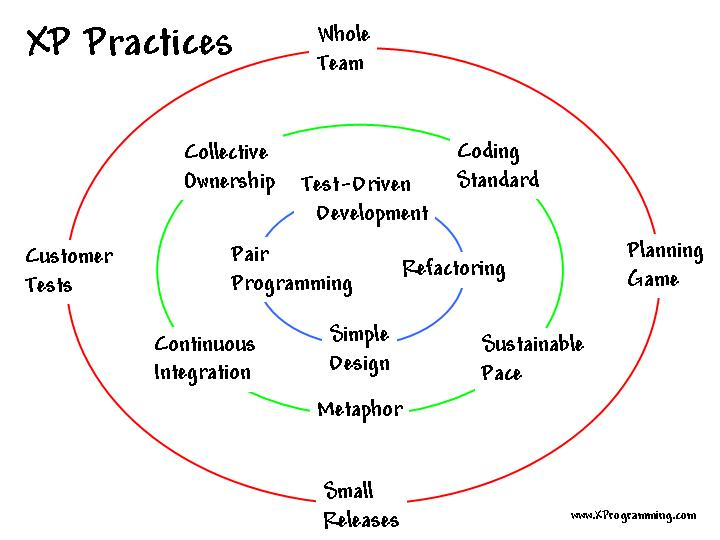
\includegraphics[width = 140mm]{circles.jpg}
\caption{Extreme Programming Model~\cite{xpCircles}}
\label{fig:xp}
\end{figure}

Critics argue that this practice suffers from unstable requirements and a lack of documentation. The addition of a customer representative as part of the development team can also create feature creep, resulting in a project which runs out of time and
money. The customer representative can also become a point of stress for the team, or a single point of failure for the entire project. Change-control boards are created to prevent this, a sign that there can be conflicts in project objectives. Many more criticisms can be found in Extreme Programming Refactored~\cite{xpRefactored}.

\subsubsection{Crystal Clear}
Crystal clear is part of a family of methodologies known as Crystal. There are several key traits to the Crystal family, Firstly projects are categorised based no there criticality and size. There are 4 levels of criticality for a project:

\begin{itemize}
\item Comfort (C)
\item Discretionary Money (D)
\item Essential Money (E)
\item Life (L)
\end{itemize}

This combined with the maximum number of people to be involved in the project make up the project category. For example a C30 project is a Comfort-Critical project involving 30 people. This rating is important as they put emphasis on communication, which is made more difficult with larger teams. As such the project category helps calculate how rigorous the approach needs to be. 

Each member of the crystal family has been given a colour which is assigned to a project category. Currently there are Clear, Yellow, Orange, Red, Maroon, Blue, and Violet versions of the crystal methodology. 

Clear is designed for projects with a rating of around C6 or D6, with other colours aimed at more complex projects (Such as Red for the E80, D80 and C80 categories). 

Each methodology follows a set of common traits:

\begin{itemize}
\item Follows the Agile principles. 
\item Iterative-Incremental process. 
\item Each increment is no longer than 4 months.
\item No support for life-critical systems.
\item No support for distributed teams. 
\item Stresses effective communication and information flow. 
\end{itemize}

Crystal Clear is targeted at C6 and D6 projects where there is only one development team. The team members should work in close proximity to each other to deliver usable software at least once every three months, though it is usually much more frequent. 

The process starts with Charting. Charting is the process of forming a team, analysing the feasibility of the project, adjusting the development methodology and making an initial plan. 

After charting comes the cyclic delivery. There is usefully two or more delivery cycles, each one taking from one week to three months. During a cycle the team should be refining the plan, implementing subsets of the requirements through program-test-integrate iterations. These sub-iterations are usually daily cycles. As the iteration comes to a close they should be delivering the integrated product to users and reviewing the development methodology and project plan.

After the cyclic delivery is complete the project is wrapped up, the product is deployed into the user environment and post-deployment reviews and reflections are undertaken. 

\begin{figure}[H]
\centering
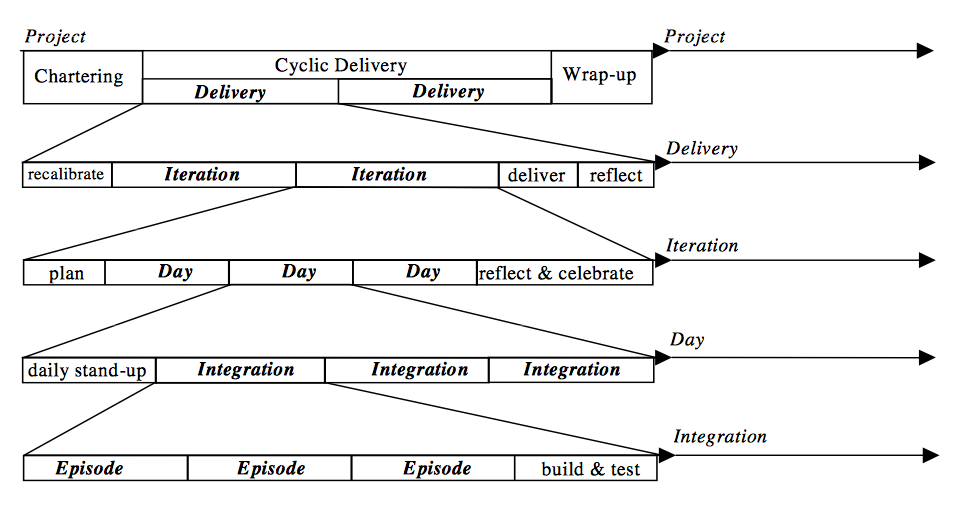
\includegraphics[width = 140mm]{clear.png}
\caption{The composition of iterations in Crystal Clear ~\cite{Cockburn}}
\label{fig:clear}
\end{figure}

Generally Crystal clear is seen as good iterative-incremental process powered by planning and reviewing. It allows for continuous integration and is flexible and configurable to a users needs. How ever it only has limited scalability and does not share a common process with other crystal methods. It is also limited by its unsuitability for highly critical and over-dependence on inter-human communication. It also depends on a more day to day and continuous development period, which would make it difficult to apply to our project. 

\subsubsection{Scrum}
Scrum is an iterative and incremental type of Agile software development that focuses on the ability of a team to work together to complete the project. It encourages co-location of all members of the team and verbal communication. 

One of the key aspects of scrum is its ability to recognise that the client may change their mind about what they need, called a requirements churn, and that unpredicted challenges are difficult to plan for and address in an traditional manor. Its because of this that scrum adopts an empirical approach. This means the team should accept that a problem cannot be fully understood or controlled and instead should focus on their ability to work quickly and respond to any newly emerging requirements. 

SCRUM defines 3 core roles to any team:

\begin{description}
\item[Product Owner] The product owner is the stakeholder and voice of the client. They are responsible for producing a valuable product and writing customer-centric items for the project backlog. This role is usually combined with the role of Project Manager, but should not be merged with the role of Scrum Master. 
\item[Development Team] The development team are responsible for delivering a working product (A Potentially Shippable Increment (PSI)) at the end of each sprint cycle. The team is usually between 3 and 9 members who carryout the analysis, planning, development, testing, etc on the project. The team is usually self-organised.
\item[Scrum Master] The scrum master is in charge of ensuring the development team can complete a sprint quickly and without impediment from external influences. They enforce the rules of SCRUM, chair key meetings and challenge the team to improve. Unlike a traditional Project Manager the Scrum Master doesn't have to deal with the management of people, only ensure the project is progressing and following the Scrum rules. 
\end{description}

One of the key aspects of SCRUM are the sprint development iterations. A sprint is a basic development iteration and is often has a fixed length. The length is often set before the sprint begins and varies between 1 week and a month. Sprints begin with a Planning meeting where the tasks are identified and an estimation of the commitment to that sprint is made. They end with a  review and retrospective meeting where the progress made is reviewed and any possible lessons from the sprint are documents for later sprints. Each meeting has a time limit, varying from 3 hours to 8 hours. At the end of each sprint the software should be fully integrated, tested and working. It should be in a 'Potentially Shippable' state. During a spring there are daily scrums which are short 15 minute meetings for the whole team to discuss the previous days work and what should be done that day. 

There are several artefacts related to SCRUM, Firstly there is a Product backlog. The product backlog is a list of requirements for the project. They are organised by the order in which they should be implemented. These requirements are usually features, bugs, non-functional requirements, etc. It is an open list and editable by anyone, but the Product Owner is ultimately responsible for ordering the items. 

As well as the Product backlog there is a Sprint Backlog which details the work the development team must complete in the next sprint. This is created by picking items from the top of the product backlog until the development team feel they have enough work to fill the sprint. Each item is broken down into tasks, which developers can sign up to work on. The sign up processes encourages the developers to be involved in the project. Once a sprint backlog is committed only the team can add to it.

The sprint method ensure that the product is regularly updated and in a working state. This can drastically decrease the time till completion for a project. The review process at the end of each sprint works to improve further sprints and improve the project as it progresses. It is actively anticipating requirement changes and is able to adapt to changing circumstances quickly and easily. Most importantly the method seeks to keep the developers involved in the project and forces them to take an interest in all stages. However the potential regular changes to requirements can result in a hectic and complicated work schedule. The frequent meetings and reviews also require a large amount of time which could potentially be spent developing the product further. 

\subsection{Chosen Development Methodology}
\label{sec:chosen-method}

The methodology which has been chosen is Scrum. From the methodologies discussed in section~\ref{sec:considered-methods} the choices were narrowed down to either Crystal Clear or Scrum due to their user focused nature and ability to adapt to change. Scrum was decided upon as it is a methodology which the majority of the team are comfortable with, or have used before. The sprints will allow for the team to keep a structured work flow throughout the project and ensure that each requirement is designed, implemented and tested before another is begun. In table~\ref{tab:scrumRoles} the team roles can be seen.

\begin{table}[H]
\centering
\begin{tabular}{|l|l|}
\hline
Adam Barrell & Product Owner \\ \hline
Thomas Milner & Scrum Master \\ \hline
Chris Lewis & Development Team Member \\ \hline
Lewis Hancock & Development Team Member \\ \hline
\end{tabular}
\caption{SCRUM Roles}
\label{tab:scrumRoles}
\end{table}

As the project leader Adam Barrell is to be Product Owner, Thomas Milner offered to act as Scrum Master and chair Scrum meetings. The remaining positions are development team members, filled in by Lewis Hancock and Chris Lewis. 

For version control the team shall be using Git (defined in section~\ref{sec:terms}), to help keep track of our backlog and what is currently in development the team shall also be using a Scrum project management tool called Target Process. This tool allows us to enter our backlog and manipulate it many useful ways. 

The initial sprint backlog can be found in section~\ref{sec:project-plan}.

\subsection{Software Testing}
Software testing is an important part of the development life-cycle. It is carried out in order to detect software failure. Identifying failure allows us to discover and amend software defects. Therefore, testing techniques will be used throughout the software's development. This will ensure:- 
\begin{itemize}
\item The software does exactly what the customer requires and meets the agreed specification. 
\item High quality software is produced.
\item The number of software bugs is significantly reduced.
\end{itemize}

For this project, several testing techniques will be employed; Unit, Regression, Functionality and Acceptance testing.

\subsubsection{Unit Testing} 
The purpose of unit testing is to examine the inner-workings of a software program. An internal outlook on the system is used in order to create test cases to run against the system. Test cases are generally formulated to cover branches, statements and paths within a unit. The term unit refers to a method of a class and therefore, unit testing will be performed on all classes of the program. This will ensure that every method produces the correct output. If a test fails, it will be comparatively easy to locate the error and then amend the code. Unit testing will be applied to classes when they are deemed complete. Each method of the class will undergo testing, hopefully ensuring 100\% coverage of the code. If a class passes all unit tests then we can be confident that the class components are correct and reliable. Performing unit tests will ensure that the code produced is correct, but it doesn't necessarily mean that the functionality provided by the software is correct. To overcome this issue, it will be necessary to perform functionality tests.

\subsubsection{Black-box Testing}
Functionality testing is essential to this project as users are constantly pressing buttons (input) in order to receive results (output). It will be carried out using ``Black-box'' testing. The purpose of black-box testing is to prevent the test engineer from viewing the implementation of the software. As its name suggests, its sole interest is the functionality of the system and, therefore, the test engineer is restricted to what a potential user would see. This allows the tester to assess the behaviour of the input/output functionality.

As no code will be made visible, the tester will create test cases based on the functional requirements and specification. These test cases will determine whether the software works together in the correct manner rather than testing parts of the system as individual units. This will ensure that the system does exactly what it is intended to do. When a new interface view has been developed, functionality tests will be applied. This will typically occur towards the end of every sprint cycle and will ensure that the functionality of the software complies with the requirements set at the beginning of the project. Functionality testing will also be applied towards the end of the project to ensure the entire system works smoothly and in the correct manner. The only issue with black-box testing is the fact that it is difficult to locate where in the code errors occur. However, this issue is reduced as errors in the code should have already been identified through unit testing.

\subsubsection{Regression Testing}
The third type of software testing that will be used is regression testing. This method of testing is used in order to uncover new software bugs that may be created due to alterations or enhancements being made to the system and can also be used to track the quality of the software's output. The purpose of regression testing is to ensure these issues don't introduce new software faults. Regression testing helps identify whether or not a change in one area of the software will affect any other areas. Regression testing will be employed by running completed tests that were previously carried out. If the behaviour of the software changes or if previous faults re-emerge, then the code can be re-examined and corrected. 

\subsubsection{Acceptance Testing}
The fourth and final testing method to be used will be acceptance testing. The general approach is to conduct tests, ensuring the software meets the requirements and specifications set out by the client. For this project, acceptance testing will be carried out by providing the client with the software after every relatively important feature has been designed and implemented. This will ensure the client approves of the product throughout the project. If the client has any issues or concerns with parts of the software then adjustments can be easily made. Monthly meeting with other members of the White Rock Trails company will also mean further software approval can take place. Both acceptance procedures will certify that the product created meets the client's requirements and also to a high quality standard.

\section{Project Plan}
\label{sec:project-plan}

\subsection{Sprint Feature Backlogs}

The requirements were used to build a set of tasks required to develop each feature of the project. These tasks were added to the backlog in the online tool and organised by feature. These task will be assigned to sprints and represent all the work necessary to complete the project. 

\subsubsection{Database}
\begin{figure}[H]
\centering
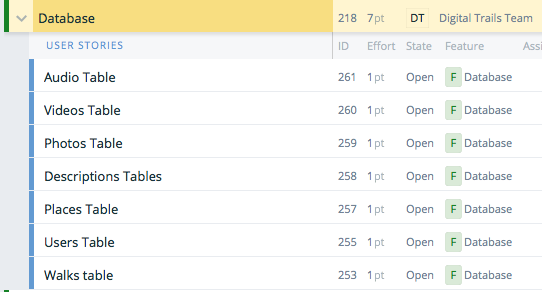
\includegraphics[width = 140mm]{backlog/Database.png}
\caption{The Database Feature Backlog.}
\label{fig:backlogDatab}
\end{figure}


\subsubsection{Application Walks}
\begin{figure}[H]
\centering
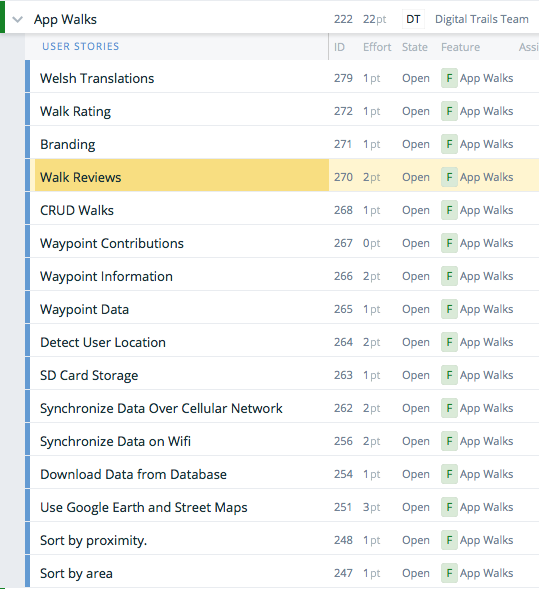
\includegraphics[width = 140mm]{backlog/AppWalks.png}
\caption{The Application Walks Feature Backlog.}
\label{fig:backlogappwal}
\end{figure}

\subsubsection{Application User}
\begin{figure}[H]
\centering
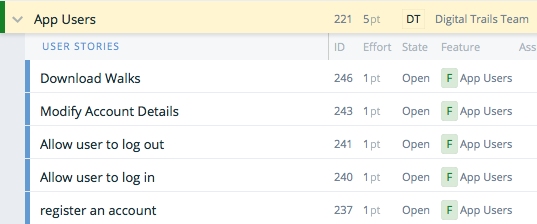
\includegraphics[width = 140mm]{backlog/AppUser.png}
\caption{The Application Users Feature Backlog.}
\label{fig:backlogappuser}
\end{figure}

\subsubsection{Application Waypoint}
\begin{figure}[H]
\centering
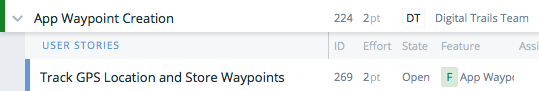
\includegraphics[width = 140mm]{backlog/AppWaypoint.png}
\caption{The Application Waypoint Feature Backlog.}
\label{fig:backlogappway}
\end{figure}

\subsubsection{Application Other}
\begin{figure}[H]
\centering
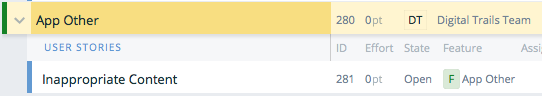
\includegraphics[width = 140mm]{backlog/AppOther.png}
\caption{Other Application Features Backlog.}
\label{fig:backlogappother}
\end{figure}

\subsubsection{Website User}
\begin{figure}[H]
\centering
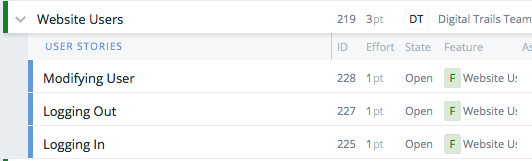
\includegraphics[width = 140mm]{backlog/WebUser.png}
\caption{The Website User Feature Backlog.}
\label{fig:backlogwebUser}
\end{figure}

\subsubsection{Website Walks}
\begin{figure}[H]
\centering
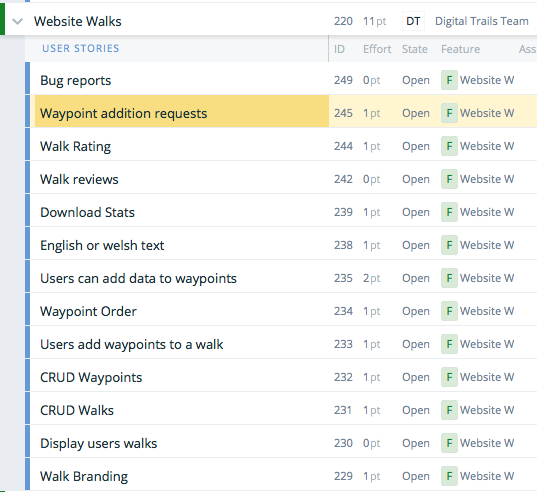
\includegraphics[width = 140mm]{backlog/WebWalks.png}
\caption{The Website Walks Feature Backlog.}
\label{fig:backlogwebwalk}
\end{figure}

\subsubsection{Website Other}
\begin{figure}[H]
\centering
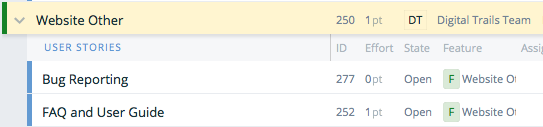
\includegraphics[width = 140mm]{backlog/WebOther.png}
\caption{The Other Website Features Backlog.}
\label{fig:backlogwebother}
\end{figure}

\subsubsection{Social Network}
\begin{figure}[H]
\centering
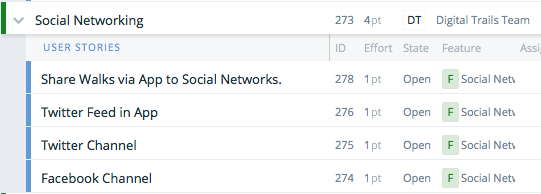
\includegraphics[width = 140mm]{backlog/Social.png}
\caption{The Social Network Features Backlog.}
\label{fig:backlogSoci}
\end{figure}

\subsection{Milestones}
\label{sec:plan-milestones}

This section will outline a timetable for the work to be completed on the formal documents of this project. Figure \ref{fig:milestones-table} shows three milestones which appear in bold font and define a set of deliverables which are to be submitted by the specified \emph{end date}. Tasks are time boxed and must be completed within the specified start and end dates if the project is to be delivered on time. Levels of indentation within the table represents that a deliverable is a child component of the higher level. For example, \emph{Design}, \emph{Testing}, \emph{User Manual}, \emph{Reflective Account} and \emph{Draft Review} are part of the \emph{Final Report} which is separate from the \emph{Project Poster} but are all deliverables for milestone 1. Milestone 1 has been planned with a higher granularity compared to milestones 2 and 3 due to the knowledge gained from the current state of development. Sections for milestones 2 and 3 cannot be planned in advance as details of future work are not fully known.

Figure \ref{fig:GanttChart} shows the timetable of milestones represented as a Gantt chart. This chart provides a clearer overview of the time boxes allocated to each task within each of the three milestones. Black directional arrows represent task dependencies whereby the task being pointed to cannot start unless all tasks pointing to it have been completed. Milestones are represented by red diamonds and tasks by rectangular blocks. Green blocks represent the review phases where the documents are reviewed prior to submission. Due to the limitations of the software used to generate the Gantt chart in Figure \ref{fig:GanttChart}, start and end dates of listed tasks are not displayed correctly.

\begin{figure}[h!]
\centering
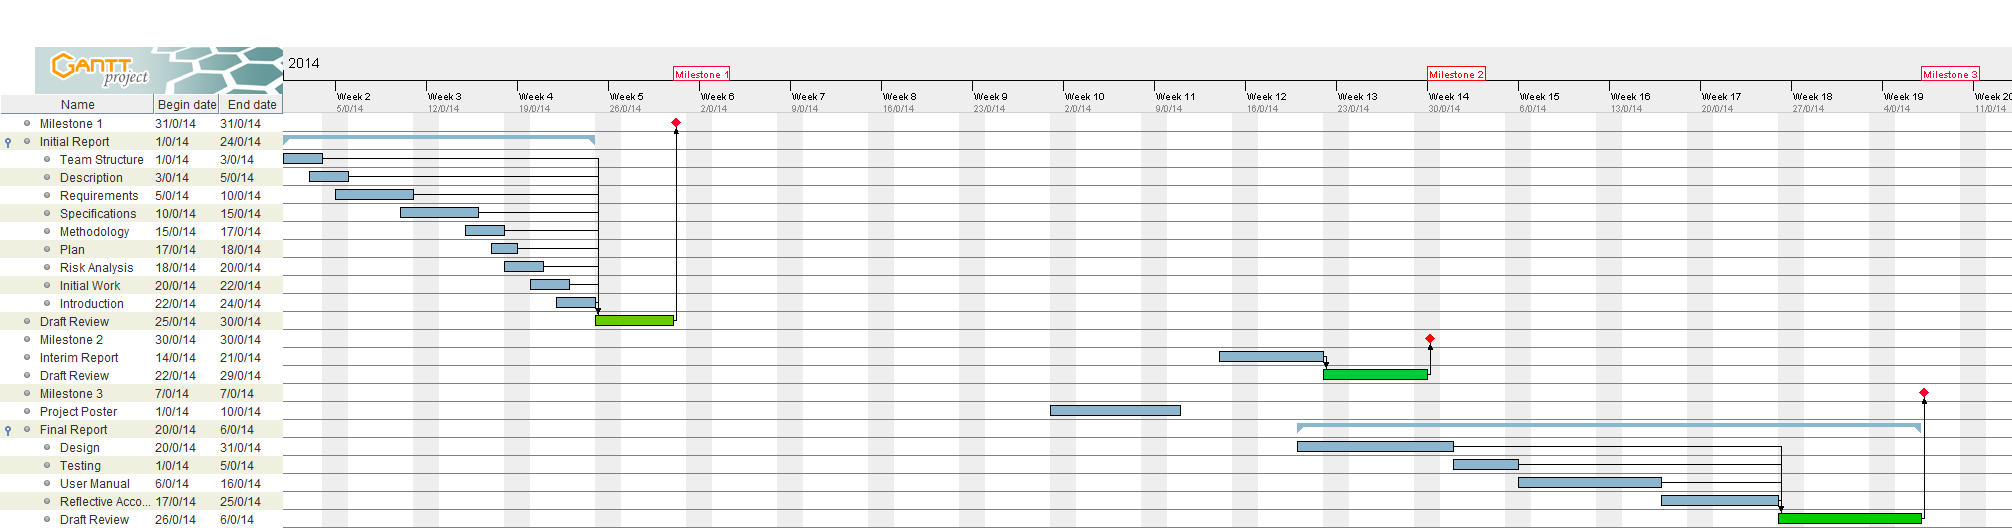
\includegraphics[angle=90,width=0.37\linewidth]{./img/GanttChart}
\caption{Gantt chart representation of milestone timetable.}
\label{fig:GanttChart}
\end{figure}


\renewcommand{\arraystretch}{1.5}
\newcommand*{\tableIndent}{\hspace*{0.4cm}}

\begin{figure}[H]
\centering
\begin{tabular}{|l|l|l|}
\hline \textbf{Task} & \textbf{Start Date} & \textbf{End Date} \\ 
\hline \hline \textbf{Milestone 1} & 01 Jan 2014 & 31 Jan 2014 \\
\hline\tableIndent Initial Report  & 01 Jan 2014 & 24 Jan 2014 \\  
\hline\tableIndent\tableIndent Team Structure  & 01 Jan 2014 & 03 Jan 2014 \\ 
\hline\tableIndent\tableIndent General Description & 03 Jan 2014 & 05 Jan 2014 \\ 
\hline\tableIndent\tableIndent Software Requirements & 05 Jan 2014 & 10 Jan 2014 \\ 
\hline\tableIndent\tableIndent Software Specifications & 10 Jan 2014 & 15 Jan 2014 \\ 
\hline\tableIndent\tableIndent Development Methodology & 15 Jan 2014 & 17 Jan 2014 \\ 
\hline\tableIndent\tableIndent Project Plan  & 17 Jan 2014 & 18 Jan 2014 \\ 
\hline\tableIndent\tableIndent Risk Analysis & 18 Jan 2014 & 20 Jan 2014 \\ 
\hline\tableIndent\tableIndent Initial Work  & 20 Jan 2014 & 22 Jan 2014 \\
\hline\tableIndent\tableIndent Introduction  & 22 Jan 2014 & 24 Jan 2014 \\  
\hline\tableIndent Draft Review  & 24 Jan 2014 & 29 Jan 2014 \\ 
\hline\textbf{Milestone 2} & 05 Mar 2014 & 28 Mar 2014 \\ 
\hline\tableIndent Interim Report & 14 Mar 2014 & 21 Mar 2014 \\ 
\hline\tableIndent Draft Review & 21 Mar 2014 & 28 Mar 2014 \\
\hline\textbf{Milestone 3} & 15 Apr 2014 & 09 May 2014 \\ 
\hline\tableIndent Project Poster & 01 Mar 2014 & 10 Mar 2014 \\ 
\hline\tableIndent Final Report & 20 Mar 2014 & 05 May 2014 \\ 
\hline\tableIndent\tableIndent Design & 20 Mar 2014 & 31 Mar 2014 \\ 
\hline\tableIndent\tableIndent Testing & 01 Apr 2014 & 05 Apr 2014 \\
\hline\tableIndent\tableIndent User Manual & 06 Apr 2014 & 16 Apr 2014 \\
\hline\tableIndent\tableIndent Reflective Account & 17 Apr 2014 & 25 Apr 2014 \\
\hline\tableIndent\tableIndent Draft Review & 25 Apr 2014 & 05 May 2014 \\
\hline 
\end{tabular}
\caption{Milestone time table.\label{fig:milestones-table}}
\end{figure}


\subsection{Software Development}
\label{sec:plan-software-dev}

This section presents the timetable that will be used for the development of the Digital Trails software. As in section \ref{sec:plan-milestones}, tasks are time boxed and given a start and end date for which they must be completed in for the project to deliver on time. However, due to the dynamic nature of sprints when using the Scrum methodology, the exact dates of each sprint cannot be defined and thus a Gantt chart cannot be generated. As the development team are using 1-2 week sprints based on the amount of work that needs to be done, an abstract time box is defined for each sprint activity. Sprints will run from the start date until the end date by which time the final software should be delivered.

Client meetings are included in this timetable because they are essential to the software development process. Important feedback is gained when the development team meets with the client to discuss and demonstrate progress. The initial three client meetings shown in Figure \ref{fig:software-dev-table} represent the sessions needed to confirm initial requirements with the client prior to development. This activity is then replaced by the \emph{client feedback} phase near the end of each sprint.

\renewcommand{\arraystretch}{1.5}

\begin{figure}[H]
\centering
\begin{tabular}{|l|l|l|}
\hline \textbf{Task} & \textbf{Start Date} & \textbf{End Date} \\ 
\hline\hline{Client Meeting 1} & \multicolumn{2}{c|}{25 Oct 2013} \\ 
\hline{Client Meeting 2} & \multicolumn{2}{c|}{15 Nov 2013} \\
\hline{Client Meeting 3} & \multicolumn{2}{c|}{14 Jan 2014} \\
\hline \multirow{2}{*}{\textbf{Sprints}} & \multicolumn{2}{c|}{1-2 Week Iterations} \\ \cline{2-3}
 & 22 Jan 2014 & 09 May 2014 \\
\hline\tableIndent{Backlog Refinement} & \multicolumn{2}{c|}{4 Hours} \\
\hline\tableIndent{Analyse} & \multicolumn{2}{c|}{4 Hours - 1 Day} \\
\hline\tableIndent{Develop} & \multicolumn{2}{c|}{3-9 Days} \\
\hline\tableIndent{Test} & \multicolumn{2}{c|}{1-2 Days} \\
\hline\tableIndent{Client Feedback} & \multicolumn{2}{c|}{4 Hours - 1 Day} \\
\hline\tableIndent{Deploy} & \multicolumn{2}{c|}{2-4 Hours} \\
\hline 
\end{tabular}
\caption{Software development time table.\label{fig:software-dev-table}}
\end{figure}

\section{Risk Analysis}
\label{sec:risk-analysis}

This section will explore the risks associated with this project. An overview of these risks is presented using a risk matrix diagram in section \ref{sec:risk-matrix}. Sections \ref{sec:tech-risks} and \ref{sec:personal-risks} discuss technical and personal risks respectively. This risk analysis will ensure project risks are foreseen and appropriate mitigation strategies are in place should any materialise.

Sections \ref{sec:tech-risks} and \ref{sec:personal-risks} analyse the technical and personal project risks respectively. Each risk is given a subjective likelihood and impact rating from the range 1 to 10, where 1 is the lowest possible likelihood/impact and 10 is the highest likelihood/impact. An overall risk rating is also assigned by calculating the result of likelihood multiplied by impact. Risks are described on the basis of how they impact the project should they occur. Finally, a mitigation strategy is discussed which aims to reduce the likelihood of the risk occurring.

\subsection{Risk Matrix}
\label{sec:risk-matrix}

This section presents the risks associated with this project in a risk matrix diagram shown in figure \ref{fig:RiskMatrix}. The risk matrix provides an overview of project risks which allow for easy identification of risk severity. The most severe risks are shown in red and tend towards the top right of the matrix which indicates a high risk rating.

Risk \texttt{TECRSK4} is shown to be the most severe, therefore it poses the highest threat as it is highly likely to occur and will severely impact the project. Risk \texttt{TECRSK4}  addresses the possible limitations of GPS hardware in the target device, the Tesco Hudle. If the GPS hardware was found to be severely limited, this would greatly impact the project as the app's location tracking would not work correctly. In addition, the project is dependent on the suitability of the Tesco Hudl as it will be the likely device used by the target audience. Risks such as these will require careful monitoring throughout the project. 

Risks tending towards the bottom left shown in green, are rated with less severity and thus do not require as careful monitoring. \texttt{PERRSK12} for example has the lowest overall risk rating and is therefore the lowest threat to the project. This risk addresses the absence of code documentation when the source is transferred from the previous development team. This risk is relatively unlikely to occur as it is standard practice for programmers to document code as it is written. If the documentation were to be absent, it would also not require a lot of time to create. Therefore, this risk has a low overall risk rating as its impact and likelihood is low.

\begin{figure}[h!]
\centering
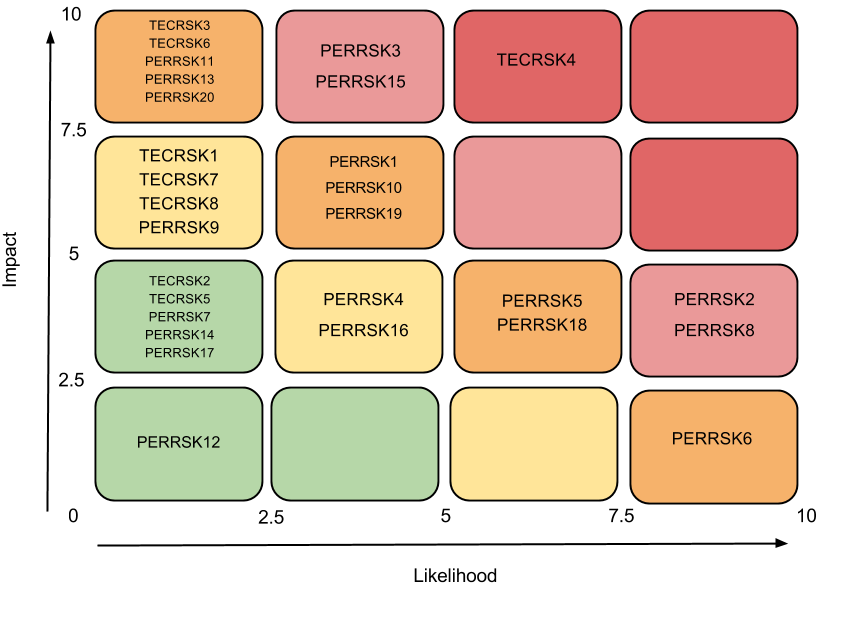
\includegraphics[width=0.9\textwidth]{./img/RiskMatrix}
\caption{Risk matrix of personal and technical project risks.}
\label{fig:RiskMatrix}
\end{figure}


\subsection{Technical Risks}
\label{sec:tech-risks}

This section explores the technical risks associated with the project. These risks are associated with the technologies which the project is dependent upon. Such risks include data loss, hardware failure, licensing issues and API limitations. \\

\renewcommand{\arraystretch}{1.2}

\noindent\begin{tabular}{@{}p{3.5cm}p{3cm}p{2.5cm}p{3cm}@{}}
\textbf{Code:} TECRSK1 & \textbf{Likelihood:} 1 & \textbf{Impact:} 7 & \textbf{Rating:} 7\\ 
\multicolumn{4}{@{}p{17cm}@{}}{\textbf{Risk:} The target tablet device, the Tesco Hudle fails and is irrecoverable to its factory state. This will prevent software testing on the target device and demonstrations to the client.} \\
\multicolumn{4}{@{}p{17cm}@{}}{\textbf{Mitigation:} Non target devices owned by members of the development team will be used to test the software and demonstrate it to the client should the target device fail.} \\
\end{tabular}

\vspace{0.5 cm}

\noindent\begin{tabular}{@{}p{3.5cm}p{3cm}p{2.5cm}p{3cm}@{}}
\textbf{Code:} TECRSK2 & \textbf{Likelihood:} 2 & \textbf{Impact:} 3 & \textbf{Rating:} 6\\ 
\multicolumn{4}{@{}p{17cm}@{}}{\textbf{Risk:} The personal computers used for software development by members of the team fail and are irrecoverable to an operational state.} \\
\multicolumn{4}{@{}p{17cm}@{}}{\textbf{Mitigation:} University lab computers with pre-installed IDE's (Integrated Development Environments) will be used to develop the software should team member's personal computers fail.} \\
\end{tabular}

\vspace{0.5 cm}

\noindent\begin{tabular}{@{}p{3.5cm}p{3cm}p{2.5cm}p{3cm}@{}}
\textbf{Code:} TECRSK3 & \textbf{Likelihood:} 2 & \textbf{Impact:} 10 & \textbf{Rating:} 20\\ 
\multicolumn{4}{@{}p{17cm}@{}}{\textbf{Risk:} Data associated with project documents and source code becomes corrupt or lost and cannot be recovered. Extra work will be required to rewrite source code and documents which will severely delay the final delivery.} \\
\multicolumn{4}{@{}p{17cm}@{}}{\textbf{Mitigation:} GIT (see terms) will be used as a version control system which will synchronise and back up source code to a remote GitHub (see terms) repository. This will ensure code is recoverable to a previous state if it becomes corrupted or lost on a single development computer.} \\
\end{tabular}

\vspace{0.5 cm}

\noindent\begin{tabular}{@{}p{3.5cm}p{3cm}p{2.5cm}p{3cm}@{}}
\textbf{Code:} TECRSK4 & \textbf{Likelihood:} 7 & \textbf{Impact:} 9 & \textbf{Rating:} 63\\ 
\multicolumn{4}{@{}p{17cm}@{}}{\textbf{Risk:} The GPS hardware on the target tablet device is not strong enough to maintain a consistent satellite signal whilst moving. This will limit the accuracy of a user's current location whilst using a walk on the app.} \\
\multicolumn{4}{@{}p{17cm}@{}}{\textbf{Mitigation:} The GPS hardware of the target device, the Tesco Hudle will be researched to ensure its capabilities are fully known. A GPS polling strategy will also be devised to ensure the app locates the user accurately, regardless of transportation.} \\
\end{tabular}

\vspace{0.5 cm}

\noindent\begin{tabular}{@{}p{3.5cm}p{3cm}p{2.5cm}p{3cm}@{}}
\textbf{Code:} TECRSK5 & \textbf{Likelihood:} 2 & \textbf{Impact:} 3 & \textbf{Rating:} 6\\ 
\multicolumn{4}{@{}p{17cm}@{}}{\textbf{Risk:} Licensing issues prevent the usage of external libraries or content for the purposes of the software that will be created. This may prevent certain resources being used in the software.} \\
\multicolumn{4}{@{}p{17cm}@{}}{\textbf{Mitigation:} The licences of potential code libraries or content will be examined before a decision is made to use them.} \\
\end{tabular}

\vspace{0.5 cm}

\noindent\begin{tabular}{@{}p{3.5cm}p{3cm}p{2.5cm}p{3cm}@{}}
\textbf{Code:} TECRSK6 & \textbf{Likelihood:} 1 & \textbf{Impact:} 8 & \textbf{Rating:} 8\\ 
\multicolumn{4}{@{}p{17cm}@{}}{\textbf{Risk:} The target tablet device, the Tesco Hudle has limited hardware which is not capable of running the developed app software responsively.} \\
\multicolumn{4}{@{}p{17cm}@{}}{\textbf{Mitigation:} Alternative tablet devices will be researched to ensure backup options are available if the Tesco Hudle is not suitable.} \\
\end{tabular}

\vspace{0.5 cm}

\noindent\begin{tabular}{@{}p{3.5cm}p{3cm}p{2.5cm}p{3cm}@{}}
\textbf{Code:} TECRSK7 & \textbf{Likelihood:} 2 & \textbf{Impact:} 7 & \textbf{Rating:} 14\\ 
\multicolumn{4}{@{}p{17cm}@{}}{\textbf{Risk:} The Google Android API is too limited to provide the functionality that is required by the app. This will result in features being excluded from the final app which cannot be developed using the standard API.} \\
\multicolumn{4}{@{}p{17cm}@{}}{\textbf{Mitigation:} Third party libraries will be researched if the standard Google Android API cannot provide the functionality required by the app.} \\
\end{tabular}

\vspace{0.5 cm}

\noindent\begin{tabular}{@{}p{3.5cm}p{3cm}p{2.5cm}p{3cm}@{}}
\textbf{Code:} TECRSK8 & \textbf{Likelihood:} 2 & \textbf{Impact:} 6 & \textbf{Rating:} 12\\ 
\multicolumn{4}{@{}p{17cm}@{}}{\textbf{Risk:} The web server used to host the web API and web portal is not of a high enough specification. This will introduce performance or compatibility issues with server side code. } \\
\multicolumn{4}{@{}p{17cm}@{}}{\textbf{Mitigation:} A suitable specification of server will be researched prior to hosting the server side code. This will be based on the volume of expected users which interact with the system at any one time.} \\
\end{tabular}

\subsection{Personal Risks}
\label{sec:personal-risks}

This section explores the personal risks associated with the project. These risks are associated with the human aspects of the project. Such risks include team member absence, feature creep, poor time management and external work. \\

\noindent\begin{tabular}{@{}p{3.5cm}p{3cm}p{2.5cm}p{3cm}@{}}
\textbf{Code:} PERRSK1 & \textbf{Likelihood:} 4 & \textbf{Impact:} 7 & \textbf{Rating:} 28 \\
\multicolumn{4}{@{}p{17cm}@{}}{\textbf{Risk:} A member of the team is absent for a substantial amount of time and is therefore not able to contribute to project work. This will cause the work rate to slow and may impact the delivery dates set out in the project timetable.} \\
\multicolumn{4}{@{}p{17cm}@{}}{\textbf{Mitigation:} Extra time will be allocated to complete project tasks so delivery dates are not severely impacted if one team member is absent. } \\
\end{tabular}

\vspace{0.5 cm}

\noindent\begin{tabular}{@{}p{3.5cm}p{3cm}p{2.5cm}p{3cm}@{}}
\textbf{Code:} PERRSK2 & \textbf{Likelihood:} 8 & \textbf{Impact:} 5 & \textbf{Rating:} 40\\ 
\multicolumn{4}{@{}p{17cm}@{}}{\textbf{Risk:} New software features are continually requested by the client after the initial requirements have been agreed. Unforeseen features will need to be allocated development time thus delaying subsequent project tasks.} \\ 
\multicolumn{4}{@{}p{17cm}@{}}{\textbf{Mitigation:} An initial set of requirements will be agreed with the client and serve as a contract. Extra feature requests will be developed if they do not impact subsequent tasks.} \\ 
\end{tabular}

\vspace{0.5 cm}

\noindent\begin{tabular}{@{}p{3.5cm}p{3cm}p{2.5cm}p{3cm}@{}}
\textbf{Code:} PERRSK3 & \textbf{Likelihood:} 5 & \textbf{Impact:} 9 & \textbf{Rating:} 45\\ 
\multicolumn{4}{@{}p{17cm}@{}}{\textbf{Risk:} The client requests the change of a feature which has already been developed. If this is a large feature such as the maps engine, a large amount of time will be required to change it, thus delaying the project timetable.} \\
\multicolumn{4}{@{}p{17cm}@{}}{\textbf{Mitigation:} Features will be prototyped and shown to the client prior to implementation. This will ensure the client agrees with the features at a user interface level.} \\
\end{tabular}

\vspace{0.5 cm}

\noindent\begin{tabular}{@{}p{3.5cm}p{3cm}p{2.5cm}p{3cm}@{}}
\textbf{Code:} PERRSK4 & \textbf{Likelihood:} 3 & \textbf{Impact:} 3 & \textbf{Rating:} 9\\ 
\multicolumn{4}{@{}p{17cm}@{}}{\textbf{Risk:} The user interface design of the web portal or app is poor causing users to struggle when using basic functions.} \\
\multicolumn{4}{@{}p{17cm}@{}}{\textbf{Mitigation:} The best practices of mobile interaction design will be adopted to ensure the app's user interface is intuitive. Neilson's design heuristics will also be applied to the web portal user interface to ensure it is also intuitive. } \\
\end{tabular}

\vspace{0.5 cm}

\noindent\begin{tabular}{@{}p{3.5cm}p{3cm}p{2.5cm}p{3cm}@{}}
\textbf{Code:} PERRSK5 & \textbf{Likelihood:} 7 & \textbf{Impact:} 3 & \textbf{Rating:} 21\\ 
\multicolumn{4}{@{}p{17cm}@{}}{\textbf{Risk:} Major or minor software bugs are present in the app or web portal which inhibit the desired functionality. This will have a negative impact on the user experience and require extra development time to fix. } \\
\multicolumn{4}{@{}p{17cm}@{}}{\textbf{Mitigation:} Blackbox testing methods such as unit and regression testing will be used at the end of each sprint to ensure modules are free from bugs. Acceptance and compatibility tests will also ensure the software is free from user interface and hardware specific bugs. } \\
\end{tabular}

\vspace{0.5 cm}

\noindent\begin{tabular}{@{}p{3.5cm}p{3cm}p{2.5cm}p{3cm}@{}}
\textbf{Code:} PERRSK6 & \textbf{Likelihood:} 8 & \textbf{Impact:} 2 & \textbf{Rating:} 16\\ 
\multicolumn{4}{@{}p{17cm}@{}}{\textbf{Risk:} The work completed by the previous development team is substandard and has left the app in an unmaintainable state. A large amount of time will be required to rewrite source code to a maintainable state. } \\
\multicolumn{4}{@{}p{17cm}@{}}{\textbf{Mitigation:} Time will be allocated for the rewriting of source code to account for previous substandard work. } \\
\end{tabular}

\vspace{0.5 cm}

\noindent\begin{tabular}{@{}p{3.5cm}p{3cm}p{2.5cm}p{3cm}@{}}
\textbf{Code:} PERRSK7 & \textbf{Likelihood:} 2 & \textbf{Impact:} 4 & \textbf{Rating:} 8\\ 
\multicolumn{4}{@{}p{17cm}@{}}{\textbf{Risk:} The team suffers from a communication breakdown where members of the team cannot be contacted or information does not circulate correctly. } \\
\multicolumn{4}{@{}p{17cm}@{}}{\textbf{Mitigation:} A communication channel will be created on a social media website which is used regularly by members of the team. This will ensure team members are always contactable and information can be distributed in one place. } \\
\end{tabular}

\vspace{0.5 cm}

\noindent\begin{tabular}{@{}p{3.5cm}p{3cm}p{2.5cm}p{3cm}@{}}
\textbf{Code:} PERRSK8 & \textbf{Likelihood:} 10 & \textbf{Impact:} 5 & \textbf{Rating:} 50\\ 
\multicolumn{4}{@{}p{17cm}@{}}{\textbf{Risk:} Team members have coursework deadlines and exam revision overlapping with project work which leaves less time to spend on development. } \\
\multicolumn{4}{@{}p{17cm}@{}}{\textbf{Mitigation:} A project timetable will be created to schedule project tasks around coursework and revision. This will ensure that sufficient time is allocated to the project. } \\
\end{tabular}

\vspace{0.5 cm}

\noindent\begin{tabular}{@{}p{3.5cm}p{3cm}p{2.5cm}p{3cm}@{}}
\textbf{Code:} PERRSK9 & \textbf{Likelihood:} 1 & \textbf{Impact:} 7 & \textbf{Rating:} 7\\ 
\multicolumn{4}{@{}p{17cm}@{}}{\textbf{Risk:} Features may be missing from the final software after it has been delivered to the client. Therefore, the client will not have the system which was specified and agreed at the start of the project. } \\
\multicolumn{4}{@{}p{17cm}@{}}{\textbf{Mitigation:} Features will be grouped and developed in multiple sprints in accordance with the Scrum development methodology. The software will also be regularly demonstrated to the client to ensure features are not missing. } \\
\end{tabular}

\vspace{0.5 cm}

\noindent\begin{tabular}{@{}p{3.5cm}p{3cm}p{2.5cm}p{3cm}@{}}
\textbf{Code:} PERRSK10 & \textbf{Likelihood:} 3 & \textbf{Impact:} 6 & \textbf{Rating:} 18\\ 
\multicolumn{4}{@{}p{17cm}@{}}{\textbf{Risk:} Software testing is not thorough enough which causes bugs to be overlooked, thus producing unintended behaviour in the software. } \\
\multicolumn{4}{@{}p{17cm}@{}}{\textbf{Mitigation:} A broad range of testing methods will be adopted such as black box, acceptance and compatibility testing to ensure unintended software behaviour is not overlooked. } \\
\end{tabular}

\vspace{0.5 cm}

\noindent\begin{tabular}{@{}p{3.5cm}p{3cm}p{2.5cm}p{3cm}@{}}
\textbf{Code:} PERRSK11 & \textbf{Likelihood:} 2 & \textbf{Impact:} 8 & \textbf{Rating:} 16\\ 
\multicolumn{4}{@{}p{17cm}@{}}{\textbf{Risk:} The developed software is slow responding to users interactions which has a negative impact on the user experience. } \\
\multicolumn{4}{@{}p{17cm}@{}}{\textbf{Mitigation:} The web portal and app will be tested on target devices to test responsiveness. Software which is not responsive enough will be redeveloped to improve its efficiency. } \\
\end{tabular}

\vspace{0.5 cm}

\noindent\begin{tabular}{@{}p{3.5cm}p{3cm}p{2.5cm}p{3cm}@{}}
\textbf{Code:} PERRSK12 & \textbf{Likelihood:} 1 & \textbf{Impact:} 1 & \textbf{Rating:} 1\\ 
\multicolumn{4}{@{}p{17cm}@{}}{\textbf{Risk:} The code documentation provided by the previous development team is substandard. This will require extra time to be invested in understanding the code and writing code documentation. } \\
\multicolumn{4}{@{}p{17cm}@{}}{\textbf{Mitigation:} Time will be allocated at the start of the project to re-factoring existing code and writing missing documentation. } \\
\end{tabular}

\vspace{0.5 cm}

\noindent\begin{tabular}{@{}p{3.5cm}p{3cm}p{2.5cm}p{3cm}@{}}
\textbf{Code:} PERRSK13 & \textbf{Likelihood:} 1 & \textbf{Impact:} 10 & \textbf{Rating:} 10\\ 
\multicolumn{4}{@{}p{17cm}@{}}{\textbf{Risk:} The software requirements defined at the start of the project are not met when the final software is delivered. Therefore, the client will not receive the software that was agreed. } \\
\multicolumn{4}{@{}p{17cm}@{}}{\textbf{Mitigation:} The client's requirements of the software will be declared in this requirements document and serve as a contract and reference. A set of specifications will also be created for each requirement to ensure tasks are set which describe how each will be achieved. } \\
\end{tabular}

\vspace{0.5 cm}

\noindent\begin{tabular}{@{}p{3.5cm}p{3cm}p{2.5cm}p{3cm}@{}}
\textbf{Code:} PERRSK14 & \textbf{Likelihood:} 1 & \textbf{Impact:} 4 & \textbf{Rating:} 4\\ 
\multicolumn{4}{@{}p{17cm}@{}}{\textbf{Risk:} The code provided by the previous development team is over engineered causing a reduction in performance and difficulties to maintain.} \\
\multicolumn{4}{@{}p{17cm}@{}}{\textbf{Mitigation:} Time will be allocated at the start of development to simplifying over engineered source code. This will ensure the code is easy to maintain and develop new features required by the client. } \\
\end{tabular}

\vspace{0.5 cm}

\noindent\begin{tabular}{@{}p{3.5cm}p{3cm}p{2.5cm}p{3cm}@{}}
\textbf{Code:} PERRSK15 & \textbf{Likelihood:} 3 & \textbf{Impact:} 9 & \textbf{Rating:} 27\\ 
\multicolumn{4}{@{}p{17cm}@{}}{\textbf{Risk:} The project plan and timetable is not robust enough to account for tasks overrunning or external factors which may delay them. This will cause an avalanche effect and disrupt the timetable.} \\
\multicolumn{4}{@{}p{17cm}@{}}{\textbf{Mitigation:} The expected time required to complete each task will be estimated with the addition of extra time incurred by predicted delays. This will ensure there is a sufficient amount of time allocated to account for task overrun.  } \\
\end{tabular}

\vspace{0.5 cm}

\noindent\begin{tabular}{@{}p{3.5cm}p{3cm}p{2.5cm}p{3cm}@{}}
\textbf{Code:} PERRSK16 & \textbf{Likelihood:} 4 & \textbf{Impact:} 4 & \textbf{Rating:} 16\\ 
\multicolumn{4}{@{}p{17cm}@{}}{\textbf{Risk:} The importance of features are over or under estimated causing more work to be spent on the less important features and less work spent on the more important features.} \\
\multicolumn{4}{@{}p{17cm}@{}}{\textbf{Mitigation:} All software features will be assigned an estimated completion time and priority which denotes the order in which they should be developed when grouped into sprints. This will ensure the correct amount of time is spent on developing tasks, starting with the most important. } \\
\end{tabular}

\vspace{0.5 cm}

\noindent\begin{tabular}{@{}p{3.5cm}p{3cm}p{2.5cm}p{3cm}@{}}
\textbf{Code:} PERRSK17 & \textbf{Likelihood:} 2 & \textbf{Impact:} 5 & \textbf{Rating:} 10\\ 
\multicolumn{4}{@{}p{17cm}@{}}{\textbf{Risk:} Members of the development team take a vacation break during project development. This leaves the rest of the team to pick up where they left off and continue their work.} \\
\multicolumn{4}{@{}p{17cm}@{}}{\textbf{Mitigation:} Members of the team who are going on a vacation break will notify the rest of the team in advance of their departure. Partially complete code will also be completed to a working state and pushed to the GitHub repository. } \\
\end{tabular}

\vspace{0.5 cm}

\noindent\begin{tabular}{@{}p{3.5cm}p{3cm}p{2.5cm}p{3cm}@{}}
\textbf{Code:} PERRSK18 & \textbf{Likelihood:} 7 & \textbf{Impact:} 4 & \textbf{Rating:} 28\\ 
\multicolumn{4}{@{}p{17cm}@{}}{\textbf{Risk:} Compatibility issues with the current code prevent the app from working correctly on the target tablet device, the Tesco Hudle. This will require more time to be spent redeveloping the code to ensure the app is compatible with the target hardware.} \\
\multicolumn{4}{@{}p{17cm}@{}}{\textbf{Mitigation:} Time will be allocated at the start of development to allow any compatibility issues to be resolved for the target tablet device. } \\
\end{tabular}

\vspace{0.5 cm}

\noindent\begin{tabular}{@{}p{3.5cm}p{3cm}p{2.5cm}p{3cm}@{}}
\textbf{Code:} PERRSK19 & \textbf{Likelihood:} 3 & \textbf{Impact:} 7 & \textbf{Rating:} 21\\ 
\multicolumn{4}{@{}p{17cm}@{}}{\textbf{Risk:} Communication with the client breaks down during the development of the software. This will prevent essential feedback from being gathered from the client, thus the final product may not be exactly as desired.} \\
\multicolumn{4}{@{}p{17cm}@{}}{\textbf{Mitigation:} An agreement with the client will be made to ensure regular contact is maintained and to inform each party of the times when they will not be contactable. } \\
\end{tabular}

\vspace{0.5 cm}

\noindent\begin{tabular}{@{}p{3.5cm}p{3cm}p{2.5cm}p{3cm}@{}}
\textbf{Code:} PERRSK20 & \textbf{Likelihood:} 1 & \textbf{Impact:} 9 & \textbf{Rating:} 9\\ 
\multicolumn{4}{@{}p{17cm}@{}}{\textbf{Risk:} The client no longer requires the software that will be developed in this project and looses interest.} \\
\multicolumn{4}{@{}p{17cm}@{}}{\textbf{Mitigation:} Regular meetings will be held with the client where the development progress will be demonstrated. Contact with the White Rock team will also be maintained to ensure their interest in the project. } \\
\end{tabular}

\section{Initial Work}
\label{sec:initial-work}
In this section meetings with the client and the initial Scrum meeting have been detailed.
\subsection{Minutes of Meetings}
Three meetings took place with the client, minutes of these meetings can be seen in Appendix A. The team has also had an initial Scrum meeting to define our backlog, the results of which can be seen in section~\ref{sec:project-plan}. 
\subsection{User Interface Wire Frames}
A set of wire-frame designs were made to help solicit feedback from the client with visual cues, thus helping clarify the requirements, these can be seen in Appendix B.

\section{Appendix A}

\lstset{basicstyle=\small, captionpos=b}

\lstinputlisting[frame=single, breaklines=true, caption=Initial Proposed Requirements]{./misc/initial-requirements.txt}

\lstinputlisting[frame=single, breaklines=true, caption=Meeting 1: 25-10-13]{./misc/25-10-13-Minutes.txt}

\lstinputlisting[frame=single, breaklines=true, caption=Meeting 2: 15-11-13]{./misc/15-11-13-Minutes.txt}

\lstinputlisting[frame=single, breaklines=true, caption=Meeting 3: 14-01-14]{./misc/14-01-14-Minutes.txt}

\section{Appendix B}

\begin{figure}[H]
\begin{center}
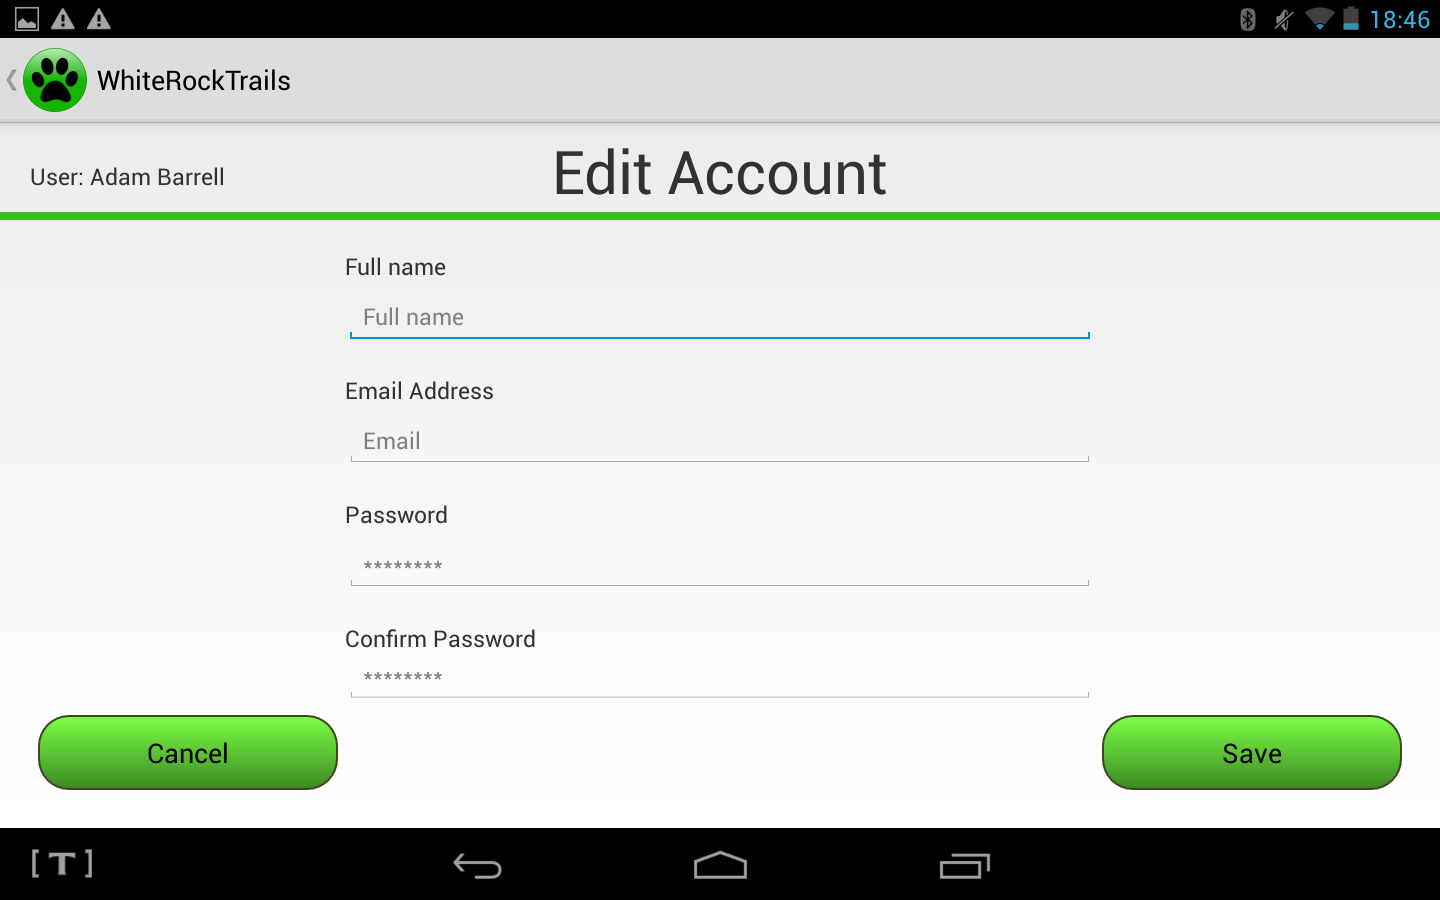
\includegraphics[scale=0.5]{account.png}
\label{fig:accountView}
\caption{The Account View}
\end{center}
\end{figure}

\begin{figure}[H]
\begin{center}
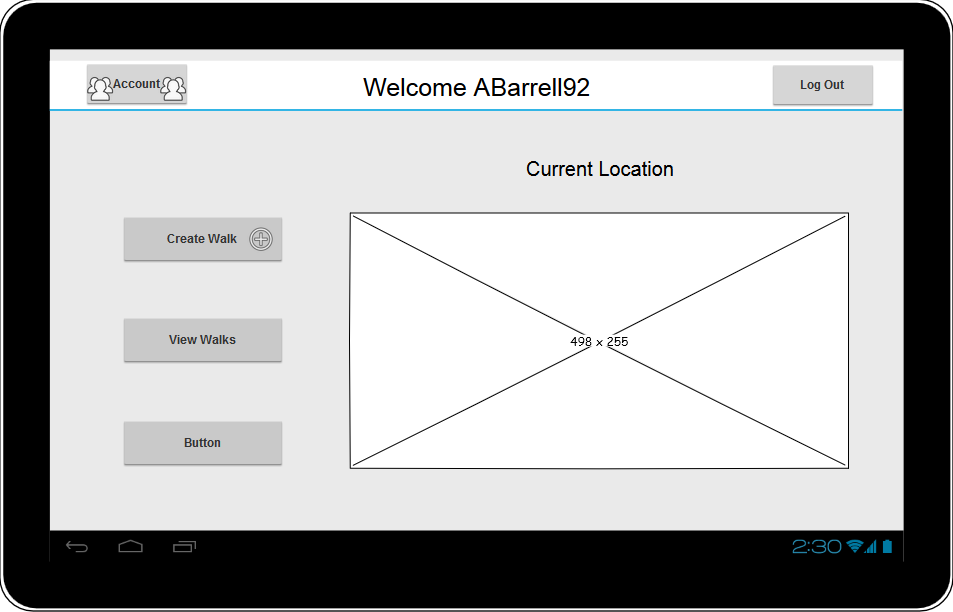
\includegraphics[scale=0.5]{HomeView.png}
\label{fig:homeView}
\caption{The Home View}
\end{center}
\end{figure}

\begin{figure}[H]
\begin{center}
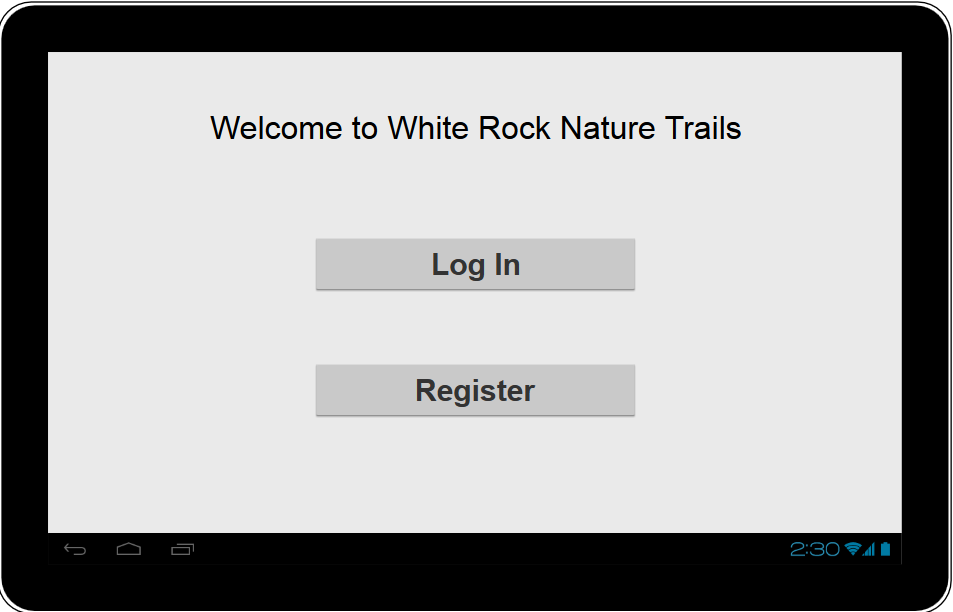
\includegraphics[scale=0.5]{LaunchView.png}
\label{fig:launchView}
\caption{The Launch View}
\end{center}
\end{figure}

\begin{figure}[H]
\begin{center}
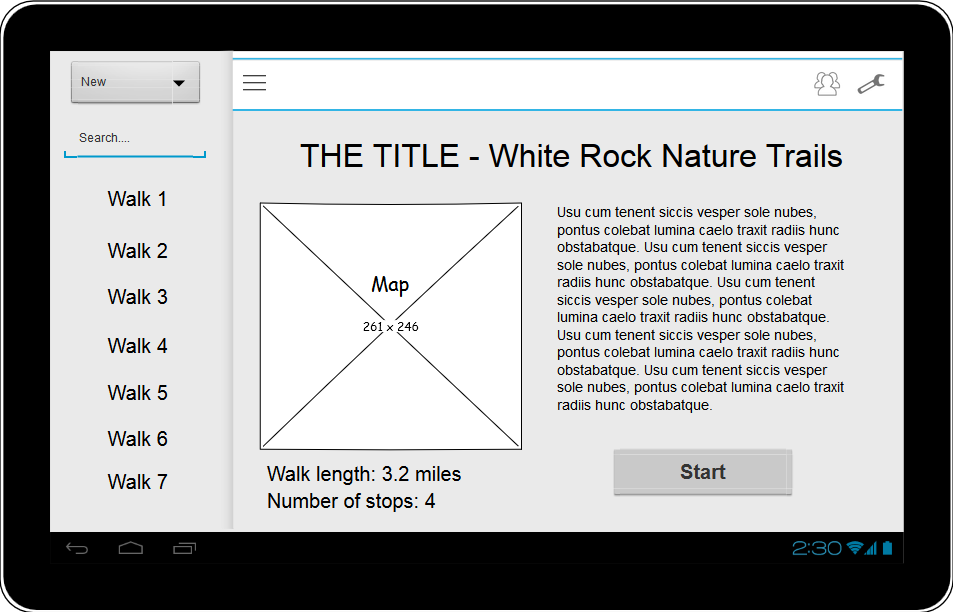
\includegraphics[scale=0.5]{ChooseAWalk.png}
\label{fig:chooseWalkView}
\caption{The Choose a Walk View}
\end{center}
\end{figure}

\begin{figure}[H]
\begin{center}
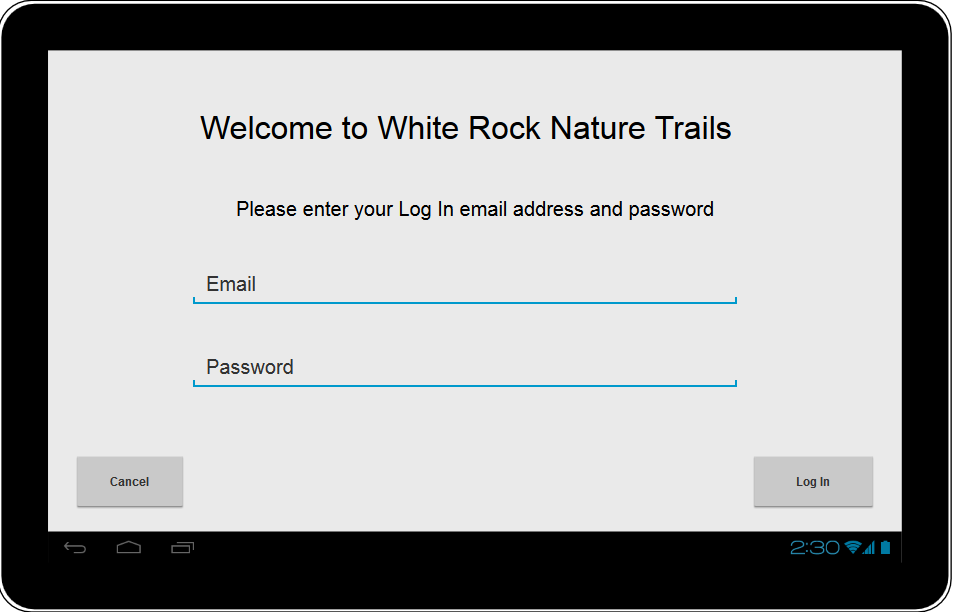
\includegraphics[scale=0.5]{LogIn.png}
\label{fig:loginView}
\caption{The Login View}
\end{center}
\end{figure}

\begin{figure}[H]
\begin{center}
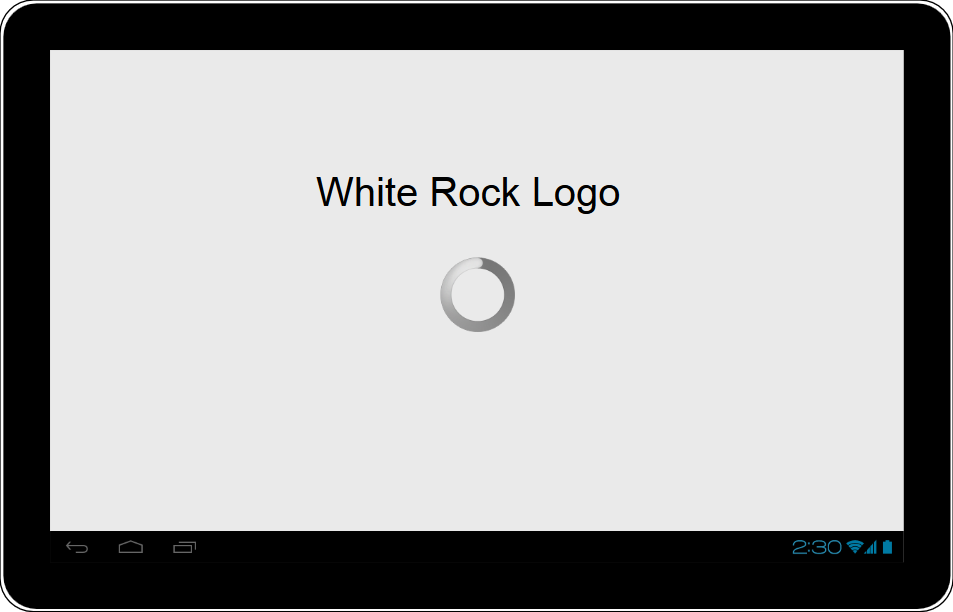
\includegraphics[scale=0.5]{SplashScreen.png}
\label{fig:splashView}
\caption{The Splash View}
\end{center}
\end{figure}

\begin{figure}[H]
\begin{center}
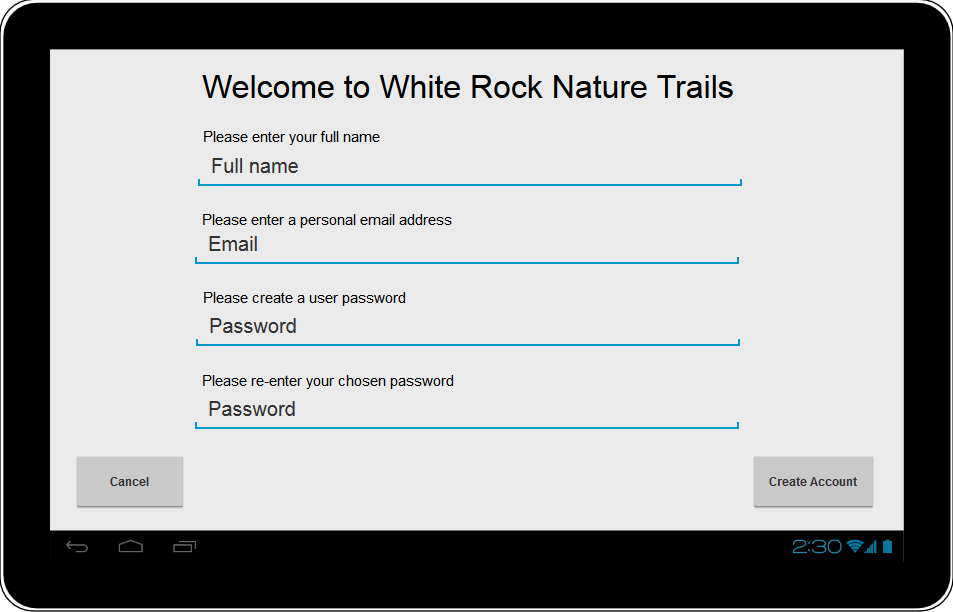
\includegraphics[scale=0.5]{Register.png}
\label{fig:registerView}
\caption{The Account Registration View}
\end{center}
\end{figure}

\begin{figure}[H]
\begin{center}
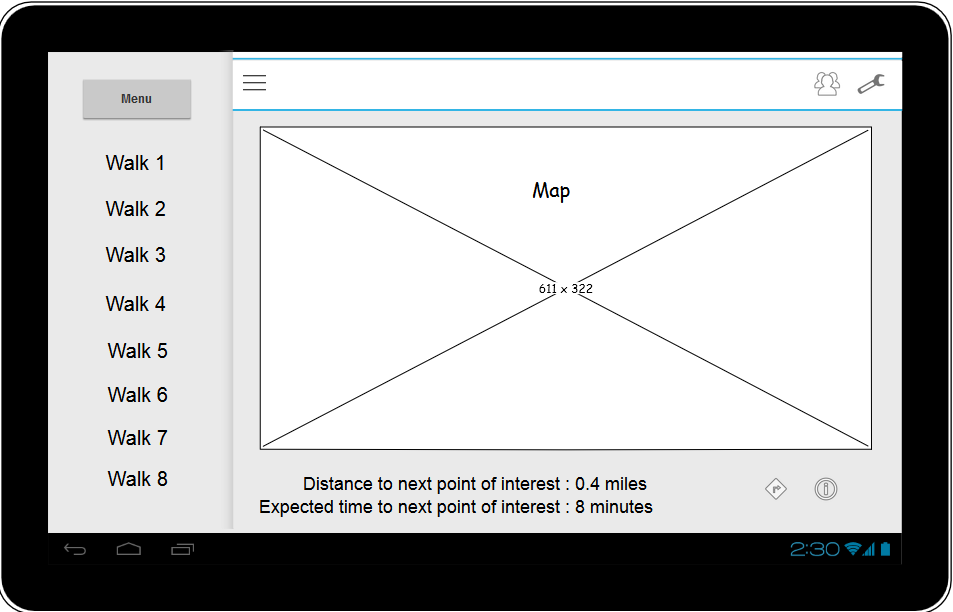
\includegraphics[scale=0.5]{WalkView.png}
\label{fig:walkView}
\caption{The Walk View}
\end{center}
\end{figure}


%References as subsection
\newpage
\bibliographystyle{plain}
\bibliography{bibliography}
\end{document}